\documentclass{ximera}

\begin{document}
	\author{Stitz-Zeager}
	\xmtitle{Equations and Inequalities involving Power Functions}


\mfpicnumber{1}

\opengraphsfile{PowerEqIneq}

\setcounter{footnote}{0}

\label{PowerEqIneq}

In this section, we set about solving equations and inequalities involving power functions.  Our first example demonstrates the usual sorts of strategies to employ when solving equations.

\begin{example} \label{powerequationex}  Solve the following equations analytically and verify your answers using a graphing utility.


\begin{multicols}{2}
\begin{enumerate}

\item \label{first} $(7-x)^{\frac{3}{2}} = 8$ 
\item \label{second} $(2t-1)^{\frac{2}{3}} -4 = 0$

\setcounter{HW}{\value{enumi}}
\end{enumerate}
\end{multicols}

\begin{multicols}{2}
\begin{enumerate}
\setcounter{enumi}{\value{HW}}

\item $(x+3)^{0.5} = 2(7-x)^{0.5}+1$ 
\item $2t^{\frac{2}{3}} + 5t^{\frac{1}{3}} = 3$

\setcounter{HW}{\value{enumi}}
\end{enumerate}
\end{multicols}


\begin{multicols}{2}
\begin{enumerate}
\setcounter{enumi}{\value{HW}}

\item $2(3x-1)^{-0.5}  = 3x (3x-1)^{-1.5}$ 
\item $6(9-t^2)^{\frac{1}{3}} = 4t^2 (9-t^2)^{-\frac{2}{3}}$

\setcounter{HW}{\value{enumi}}
\end{enumerate}
\end{multicols}

{\bf Solution.}

\begin{enumerate}

\item  One way to proceed to solve  $(7-x)^{\frac{3}{2}} = 8$ is to use Definition \ref{rationalexponentdefna} to rewrite $(7-x)^{\frac{3}{2}}$ as either $(\sqrt{7-x})^3$ or $\sqrt{(7-x)^3}$.  We opt for the former since, thinking ahead,  $8$ is a perfect cube: 

\[ \begin{array}{rclr}

(7-x)^{\frac{3}{2}} & = & 8 & \\

(\sqrt{7-x})^3 & = & 8 & \text{rewrite using Definition \ref{rationalexponentdefna}} \\

\sqrt[3]{(\sqrt{7-x})^3} & = & \sqrt[3]{8} & \text{extract cube roots}  \\

\sqrt{7-x} & = & 2 & \text{$\sqrt[3]{u^3}= u$} \\ \end{array} \]

From $\sqrt{7-x} =  2$, we square both sides and obtain $7-x = 4$, so $x = 3$.  We verify our answer analytically by substituting $x=3$ into the original equation and it checks.

Geometrically, we are looking for where the graph of $f(x) = (7-x)^{\frac{3}{2}}$ intersects the graph of $g(x) = 8$.  While we could sketch both curves by hand and gauge the reasonableness of the result,\footnote{consider this an exercise!} we are instructed to use a graphing utility.  Below on the left and see the intersection point of both graphs is $(3,8)$, thereby checking our solution $x = 3$.

\item  Proceeding similarly to the above, to solve $(2t-1)^{\frac{2}{3}} -4 = 0$, we rewrite $(2t-1)^{\frac{2}{3}}$ as $(\sqrt[3]{2t-1})^2$ and solve:

\[ \begin{array}{rclr}
(2t-1)^{\frac{2}{3}} -4  & = & 0 & \\

(\sqrt[3]{2t-1})^2 - 4 & = & 0 & \text{rewrite using Definition \ref{rationalexponentdefna}} \\
(\sqrt[3]{2t-1})^2 & = & 4 & \text{isolate the variable term} \\

\sqrt{(\sqrt[3]{2t-1})^2 } & = & \sqrt{4} & \text{extract square roots} \\

|\sqrt[3]{2t-1}| & = & 2 & \text{$\sqrt{u^2} = |u|$} \\

\sqrt[3]{2t-1} & = & \pm 2 & \text{ for $c>0$, $|u| = c$ is equivalent to $u = \pm c$.} \end{array} \]

From $\sqrt[3]{2t-1}  = 2$ we cube both sides and obtain $2t-1 = 8$, so $t = \frac{9}{2} = 4.5$.  Similarly, from $\sqrt[3]{2t-1}  = -2$, we cube both sides and obtain $2t-1 = -8$, so $t = -\frac{7}{2} = -3.5$.  Both of these solutions check in the given equation.

In this case we are looking for where the graph of $f(t) = (2t-1)^{\frac{2}{3}} -4$ intersects the graph of $g(t) = 0$ - i.e., the $t$-intercepts of the graph of $g$.  We find these are $(-3.5,0)$ and $(4.5,0)$, as predicted.

\begin{center}

\begin{tabular}{cc}

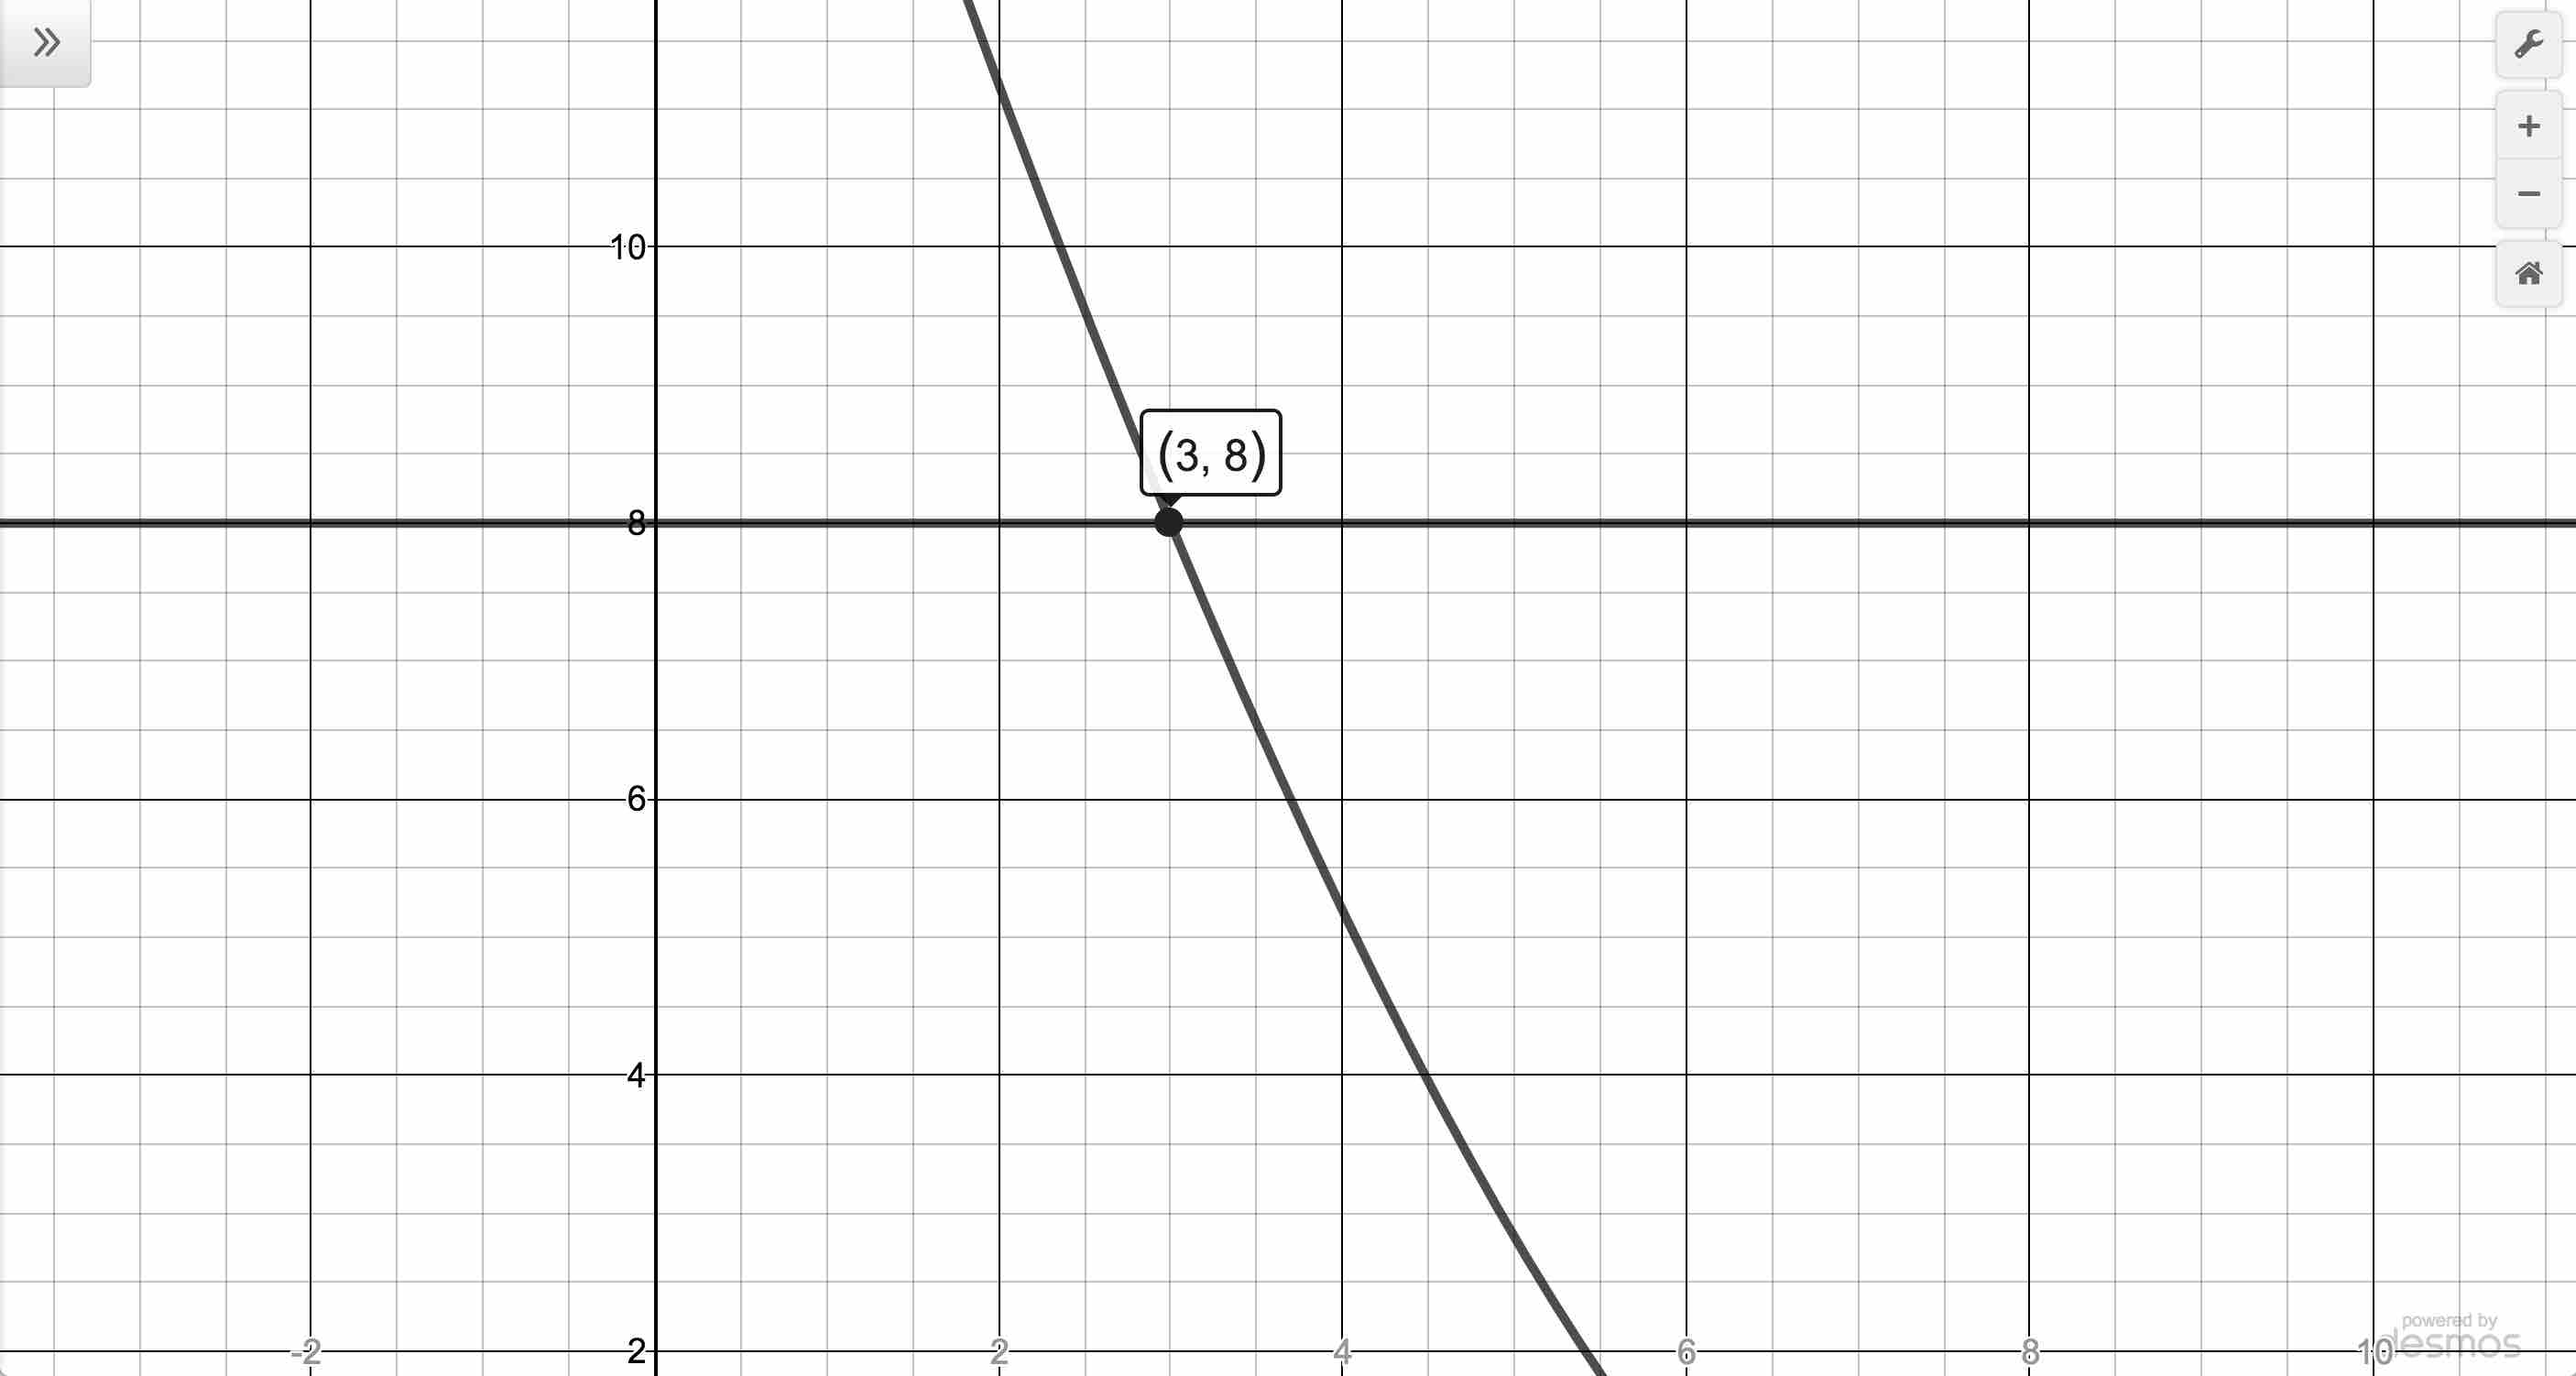
\includegraphics[width=3in]{./PowerEqIneqGraphics/PowerEqEx01.jpg} & 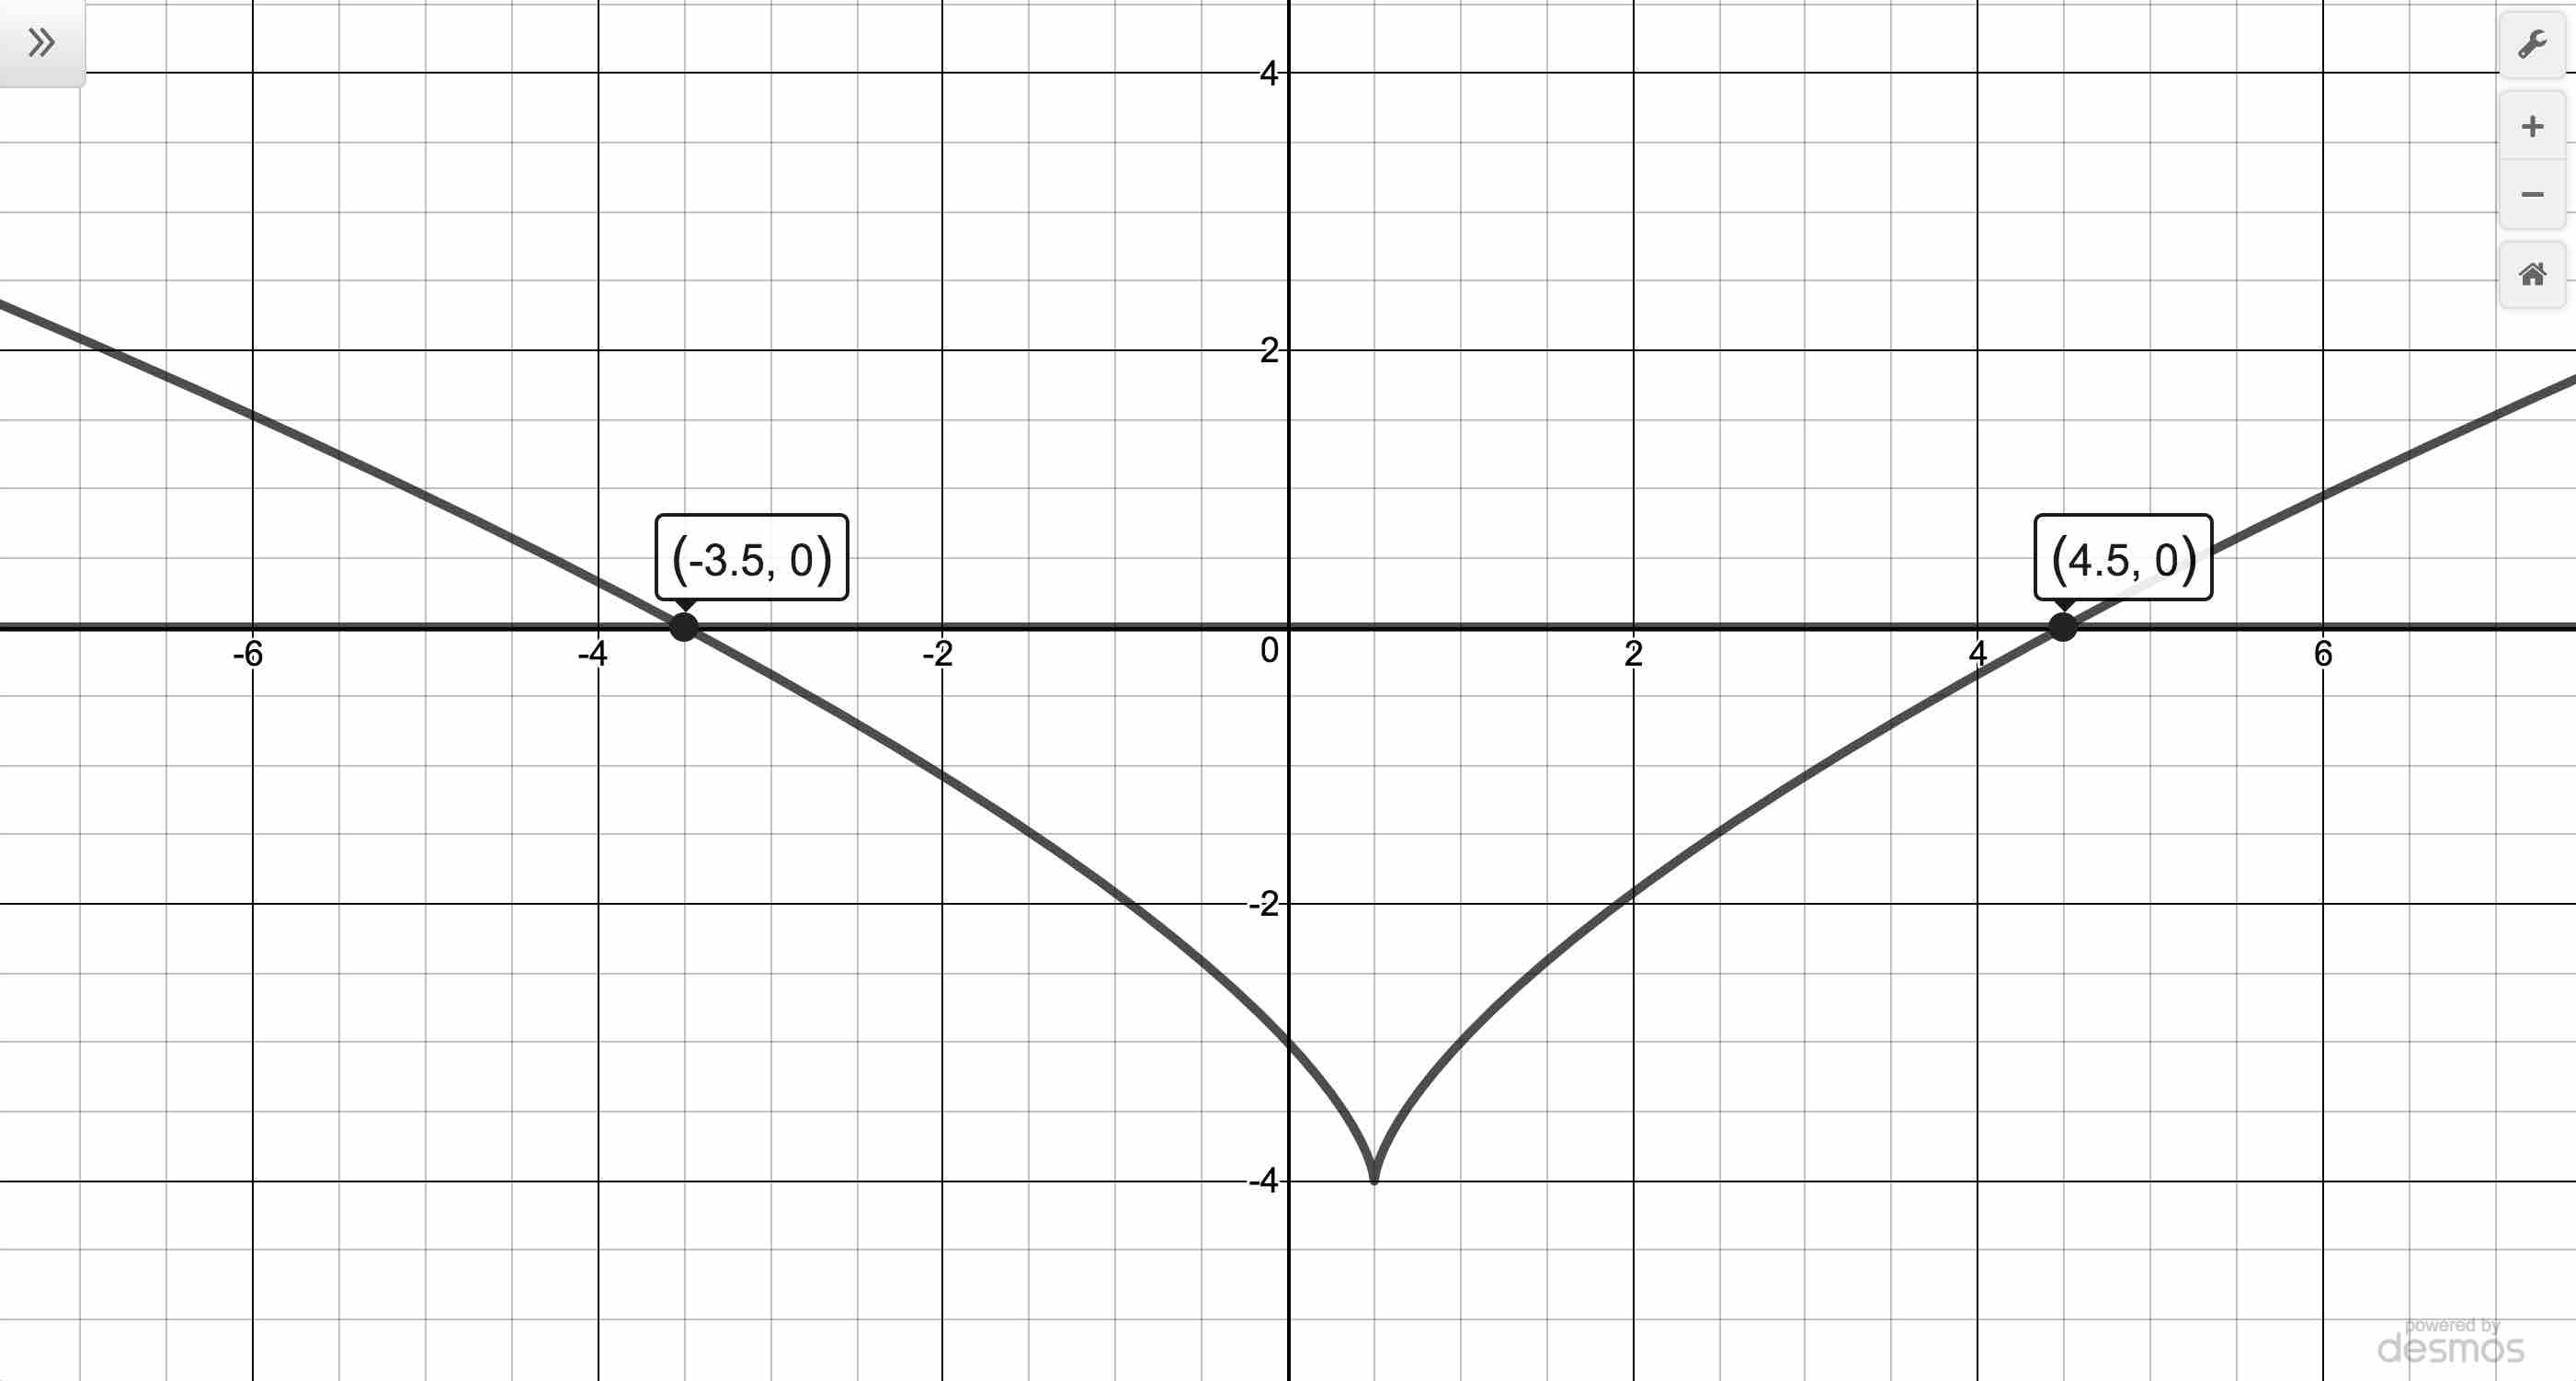
\includegraphics[width=3in]{./PowerEqIneqGraphics/PowerEqEx02.jpg} \\

Checking $(7-x)^{\frac{3}{2}} = 8$  & Checking  $(2t-1)^{\frac{2}{3}} -4 = 0$ \\

\end{tabular}

\end{center} 

\item Since $0.5 = \frac{1}{2}$, we may rewrite $(x+3)^{0.5} = 2(7-x)^{0.5}+1$ as  $(x+3)^{\frac{1}{2}} = 2(7-x)^{\frac{1}{2}}+1$.  Using Definition \ref{rationalexponentdefna}, we then have $\sqrt{x+3} = 2\sqrt{7-x} + 1$.  Since one of the square roots is already isolated, we can rid ourselves of it by squaring both sides.

\[ \begin{array}{rclr}

\sqrt{x+3} & = & 2\sqrt{7-x} + 1 & \\

 (\sqrt{x+3})^2 & = & (2\sqrt{7-x} + 1)^2 & \text{square both sides} \\
 
 x+3 & = & (2 \sqrt{7-x})^2 + 2 (2 \sqrt{7-x})(1) + 1 & \text{$(\sqrt{u})^2 = u$ and $(a+b)^2 = a^2 + 2ab +b^2$} \\

 
 x+3 & = & 4(7-x) + 4\sqrt{7-x} + 1 &  \text{$(ab)^2 = a^2b^2$ and, again, $(\sqrt{u})^2 = u$} \\
 
 x+3 & = & 28-4x+4\sqrt{7-x} + 1 & \\
 
 5x-26 & = & 4\sqrt{7-x} & \text{isolate $\sqrt{7-x}$} \\ \end{array} \]
 
We square both sides \textit{again} and get $(5x-26)^2 = (4\sqrt{7-x})^2$ which reduces to $25x^2-260x+676 = 16(7-x)$. At last, we have a quadratic equation which we can solve by setting to zero and factoring.  We get  $25x^2-244x+564 = 0$, so $(x-6)(25x-94) = 0$ so $x = 6$ or $x = \frac{94}{25} = 3.76$.  When we go to check these answers, we find $x=6$ does check, but $x = 3.76$ does not. Hence, $x=3.76$ is an `extraneous' solution.\footnote{We invite the reader to see at which point in our machinations $x=3.76$ \textit{does} check.  Knowing a solution is extraneous is one thing;  understanding \textit{how} it came about is another.}

We graph both $f(x) = \sqrt{x+3}$ and $g(x) = 2\sqrt{7-x} + 1$ below (once again, we could graph these by hand!) and confirm there is only one intersection point, $(6,3)$.

\item  While we \textit{could} approach solving  $2t^{\frac{2}{3}} + 5t^{\frac{1}{3}} = 3$ as the previous example, we would encounter cubing binomials\footnote{that is, expanding things like $(a+b)^3$.} which we would prefer to avoid.  Instead, we take a step back and notice there are three terms here with the exponent on one term, $t^{\frac{2}{3}}$ exactly twice the exponent on another term, $t^{\frac{1}{3}}$.  We have ourselves a `quadratic in disguise.'\footnote{See Section \ref{AppQuadEqus} or, more recently, Example \ref{polyquadinform} in Section \ref{RealZeros}.} To help us see the forest for the trees, we let $u = t^{\frac{1}{3}}$ so that $u^2 = t^{\frac{2}{3}}$. (Note that since root here, $3$, is odd, we can use the properties of exponents stated in Theorem \ref{exponentprops}.)  Hence, in terms of $u$, the equation   $2t^{\frac{2}{3}} + 5t^{\frac{1}{3}} = 3$ becomes the quadratic $2u^2 + 5u = 3$, or $2u^2 + 5u - 3 = 0$.  Factoring gives $(2u-1)(u+3) = 0$ so $u = t^{\frac{1}{3}} = \frac{1}{2}$ or $u = t^{\frac{1}{3}} = -3$.  Since $t^{\frac{1}{3}} = \sqrt[3]{t}$, we solve both equations by cubing both sides to get $t = \frac{1}{8} = 0.125$ and $t = -27$.  Both of these solutions check in our original equation.  Looking at the graphs of $f(t) = 2t^{\frac{2}{3}} + 5t^{\frac{1}{3}}$ and $g(t) = 3$, we find two intersection points, $(-27,3)$ and $(0.125,3)$, as required.

\begin{center}

\begin{tabular}{cc}

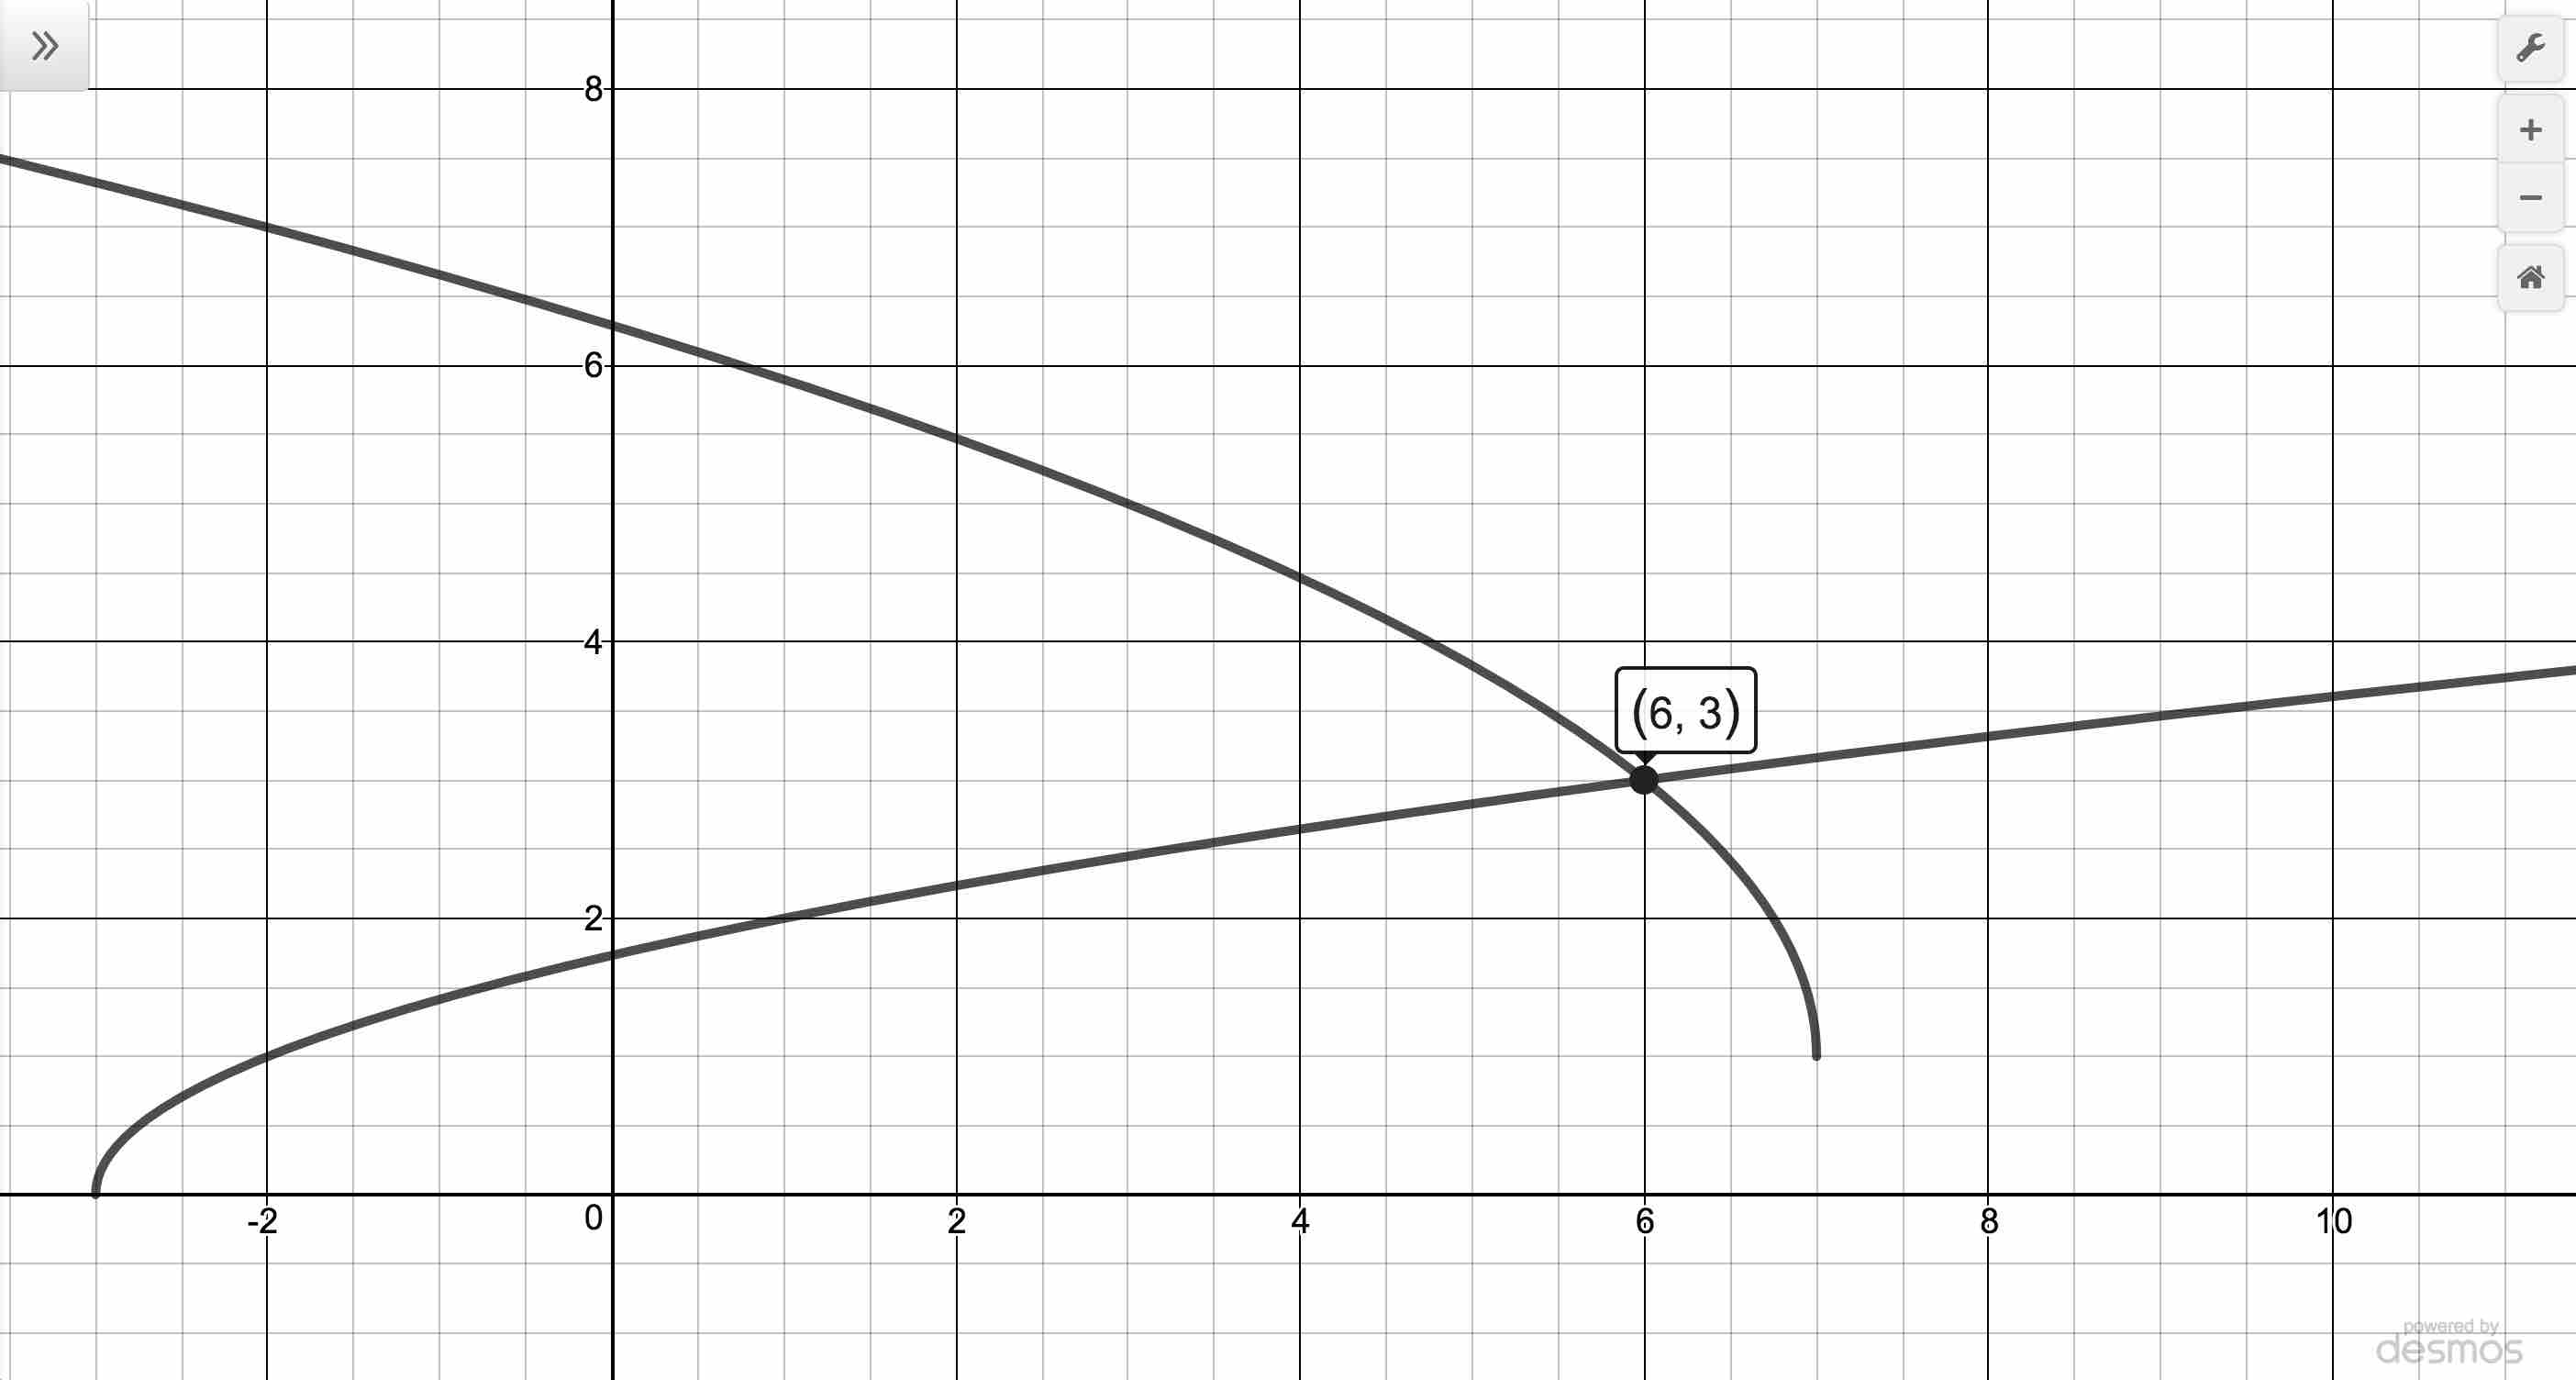
\includegraphics[width=3in]{./PowerEqIneqGraphics/PowerEqEx03.jpg} & 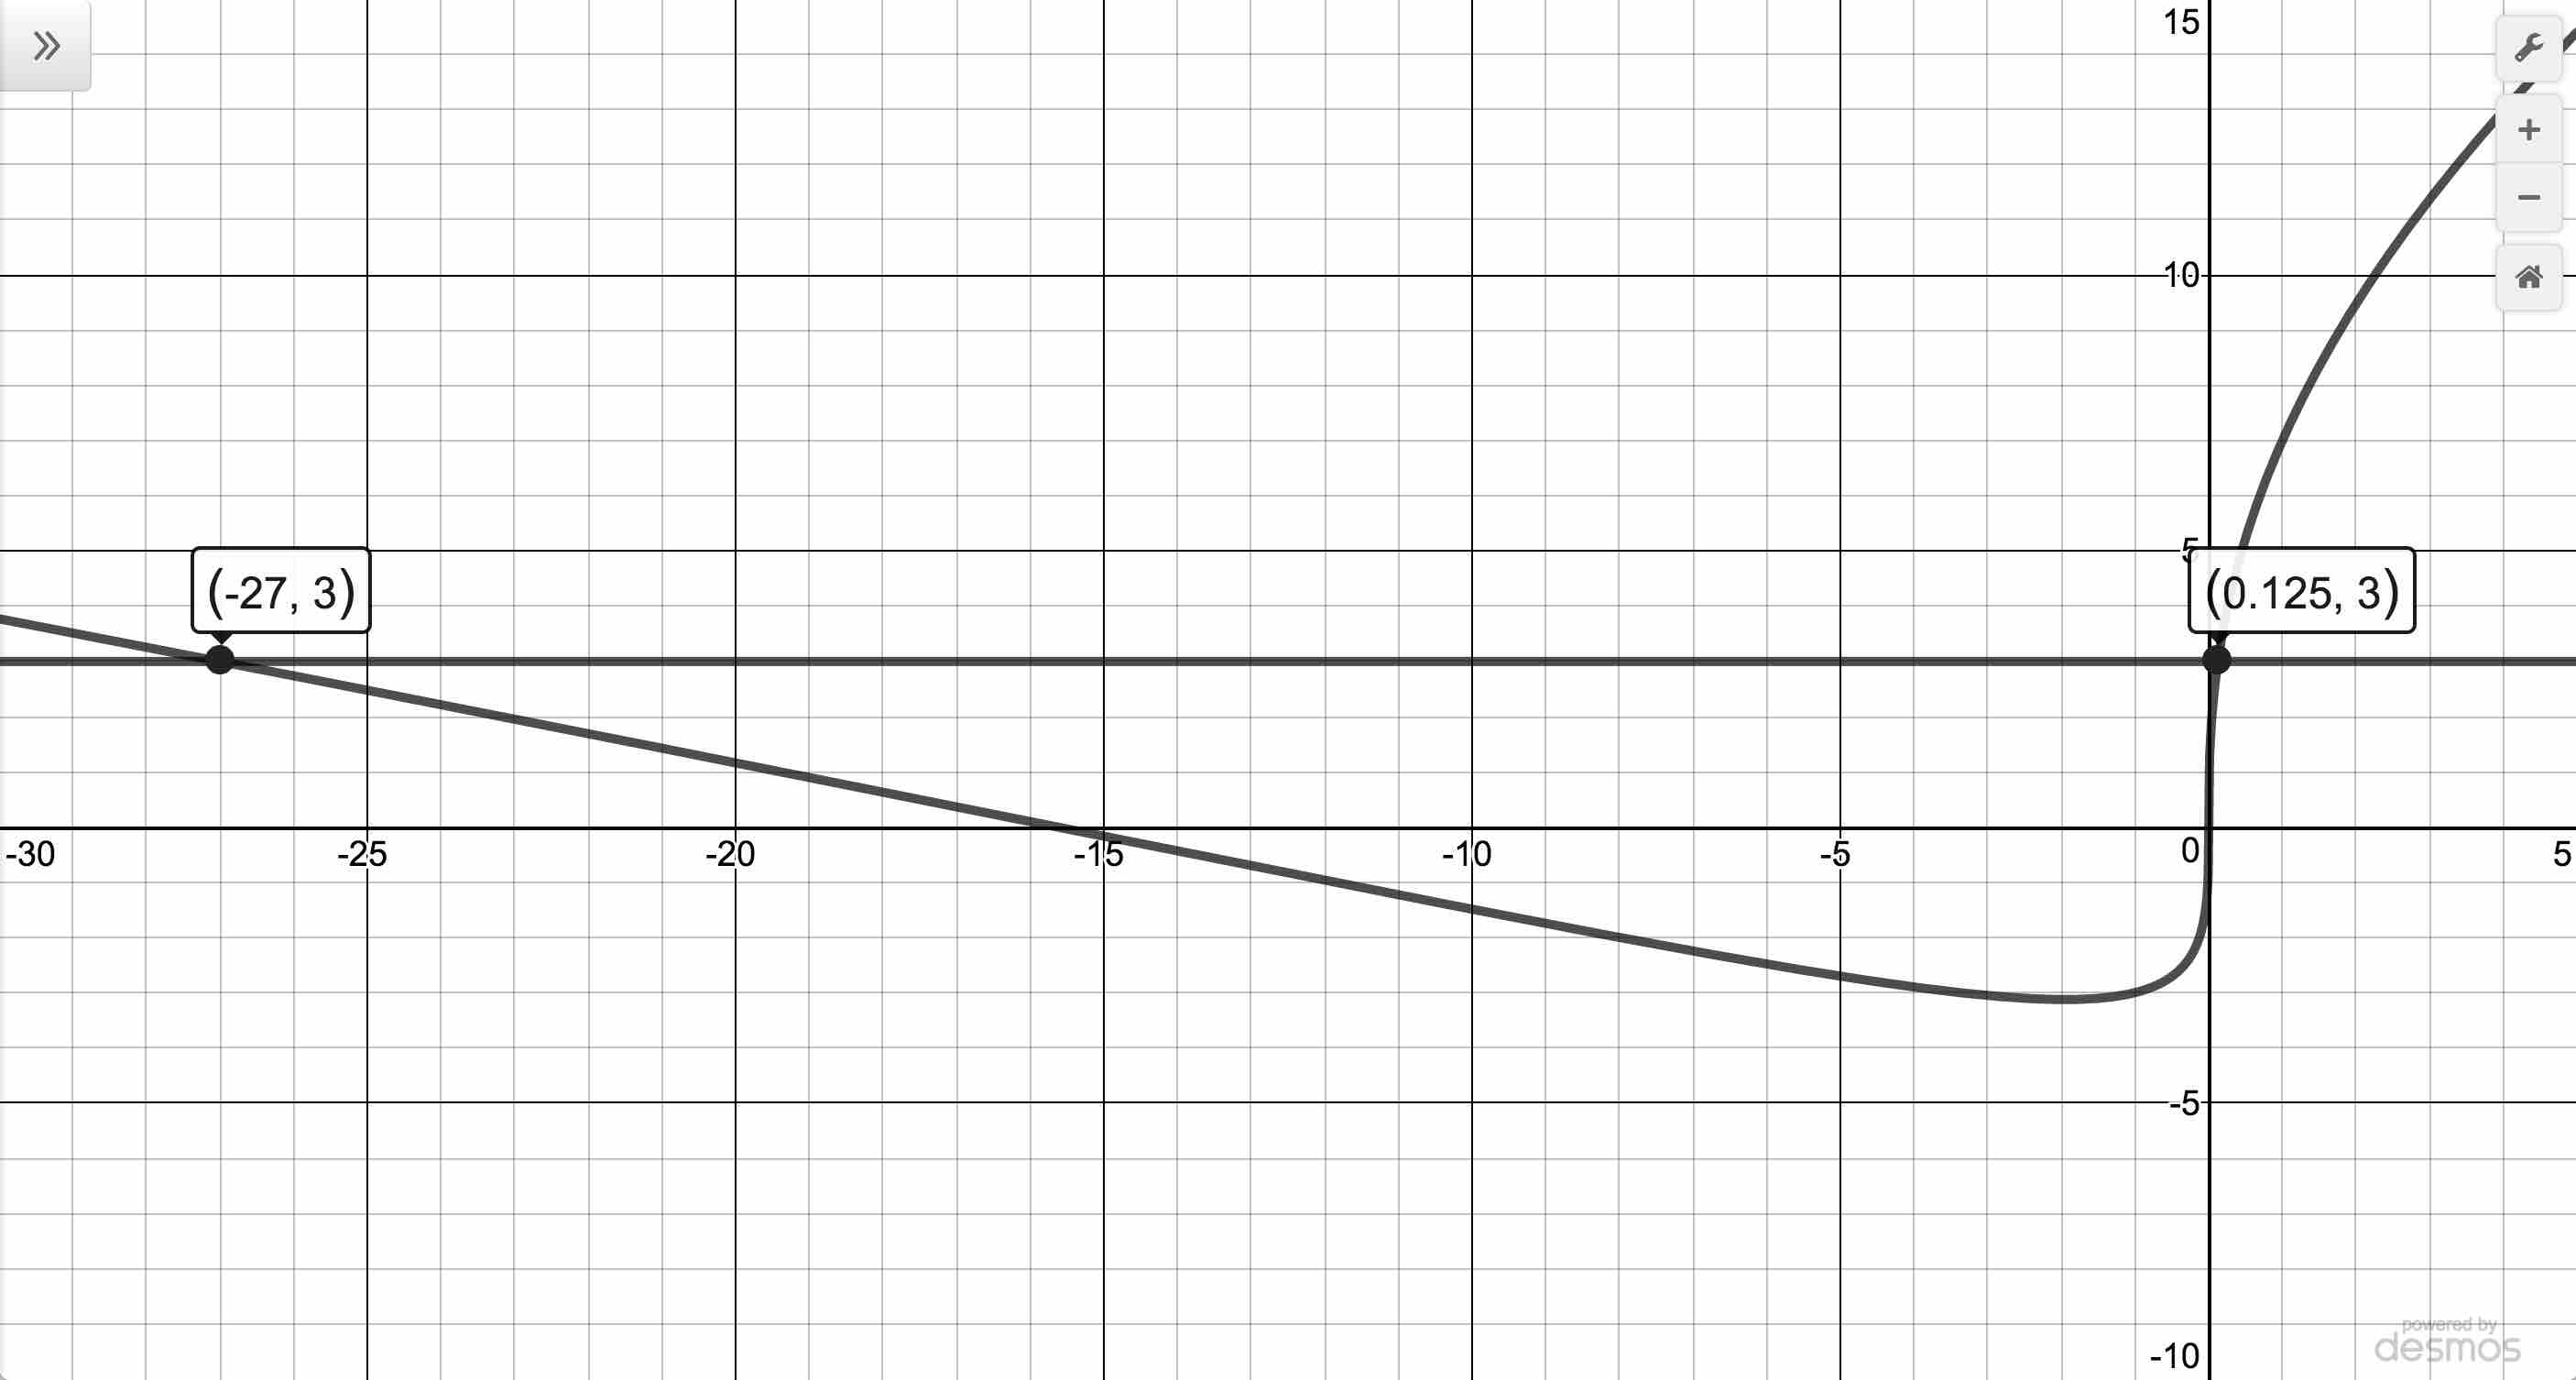
\includegraphics[width=3in]{./PowerEqIneqGraphics/PowerEqEx04.jpg} \\

Checking $(x+3)^{0.5} = 2(7-x)^{0.5}+1$ & Checking  $2t^{\frac{2}{3}} + 5t^{\frac{1}{3}} = 3$ \\

\end{tabular}

\end{center} 


\item Next we are to solve $2(3x-1)^{-0.5}  = 3x (3x-1)^{-1.5}$ which, when written without negative exponents is: $\frac{2}{(3x-1)^{0.5}} = \frac{3x}{(3x-1)^{1.5}}$.  Since the rational exponents here are $0.5 = \frac{1}{2}$ and $1.5 = \frac{3}{2}$, both involve an \textit{even} indexed root (the square root in this case!) which means $3x-1 \geq 0$.  Moreover, since the $3x-1$ resides in the \textit{denominator} $3x - 1 \neq 0$ so our equation is really valid only for values of $x$ where $3x-1>0$ or $x > \frac{1}{3}$.  Hence, we clear denominators and can apply Theorem \ref{exponentprops}:

\[ \begin{array}{rclr}

\dfrac{2}{(3x-1)^{0.5}} & = & \dfrac{3x}{(3x-1)^{1.5}} & \\

\left[ \dfrac{2}{(3x-1)^{0.5}} \right] \cdot (3x-1)^{1.5} & = & \left[  \dfrac{3x}{(3x-1)^{1.5}} \right ] \cdot (3x-1)^{1.5} & \\

2 \cdot \dfrac{(3x-1)^{1.5}}{(3x-1)^{0.5}} & = & 3x & \\

2 (3x-1)^{1.5-0.5} & = & 3x & \text{Theorem \ref{exponentprops} applies since $3x-1 > 0$.} \\

2 (3x-1)^{1} & = & 3x & \\  \end{array} \]

We get $6x-2 = 3x$, or $x = \frac{2}{3}$.  Since $x = \frac{2}{3} > \frac{1}{3}$, we keep it and, sure enough, it  checks in our original equation. Graphically we see $f(x)=2(3x-1)^{-0.5}$ intersects $g(x) = 3x (3x-1)^{-1.5}$ at the point $(0.6667, 2)$ which is the graphing utility's way of representing $\left(\frac{2}{3}, 2\right)$.

\item  Our last equation to solve is $6(9-t^2)^{\frac{1}{3}} = 4t^2 (9-t^2)^{-\frac{2}{3}}$, which, when rewritten without negative exponents is: $6(9-t^2)^{\frac{1}{3}} = \frac{4t^2}{(9-t^2)^{\frac{2}{3}}}$  .   Again, the root here ($3$) is odd, so we can use the exponent properties listed in Theorem \ref{exponentprops}.   We begin by clearing denominators: 


\[ \begin{array}{rclr}

6(9-t^2)^{\frac{1}{3}} & = & \frac{4t^2}{(9-t^2)^{\frac{2}{3}}} & \\

6(9-t^2)^{\frac{1}{3}} \cdot (9-t^2)^{\frac{2}{3}} & = & \left[   \frac{4t^2}{(9-t^2)^{\frac{2}{3}}}  \right ] \cdot (9-t^2)^{\frac{2}{3}} & \\

6(9-t^2)^{\frac{1}{3} + \frac{2}{3}}& = & 4t^2 &  \text{Theorem \ref{exponentprops} applies since the root here $3$ is odd.} \\

6(9-t^2)^{1} & = & 4t^2 &\\   \end{array} \]

We get $54 - 6t^2 = 4t^2$ or $10t^2 = 54$.  As fraction $t^2 = \frac{54}{10} = \frac{27}{5}$ so $t = \pm \sqrt{\frac{27}{5}} = \pm 3 \sqrt{15}{5}$.  While not the easiest to check analytically, both of these solutions do work in the original equation.  Graphing $f(t) = 6(9-t^2)^{\frac{1}{3}} $ and $g(t) =  4t^2 (9-t^2)^{-\frac{2}{3}}$ below, we see the graphs intersect when $t \approx \pm 2.324$ which are decimal approximations of our exact answers.

\begin{center}

\begin{tabular}{cc}

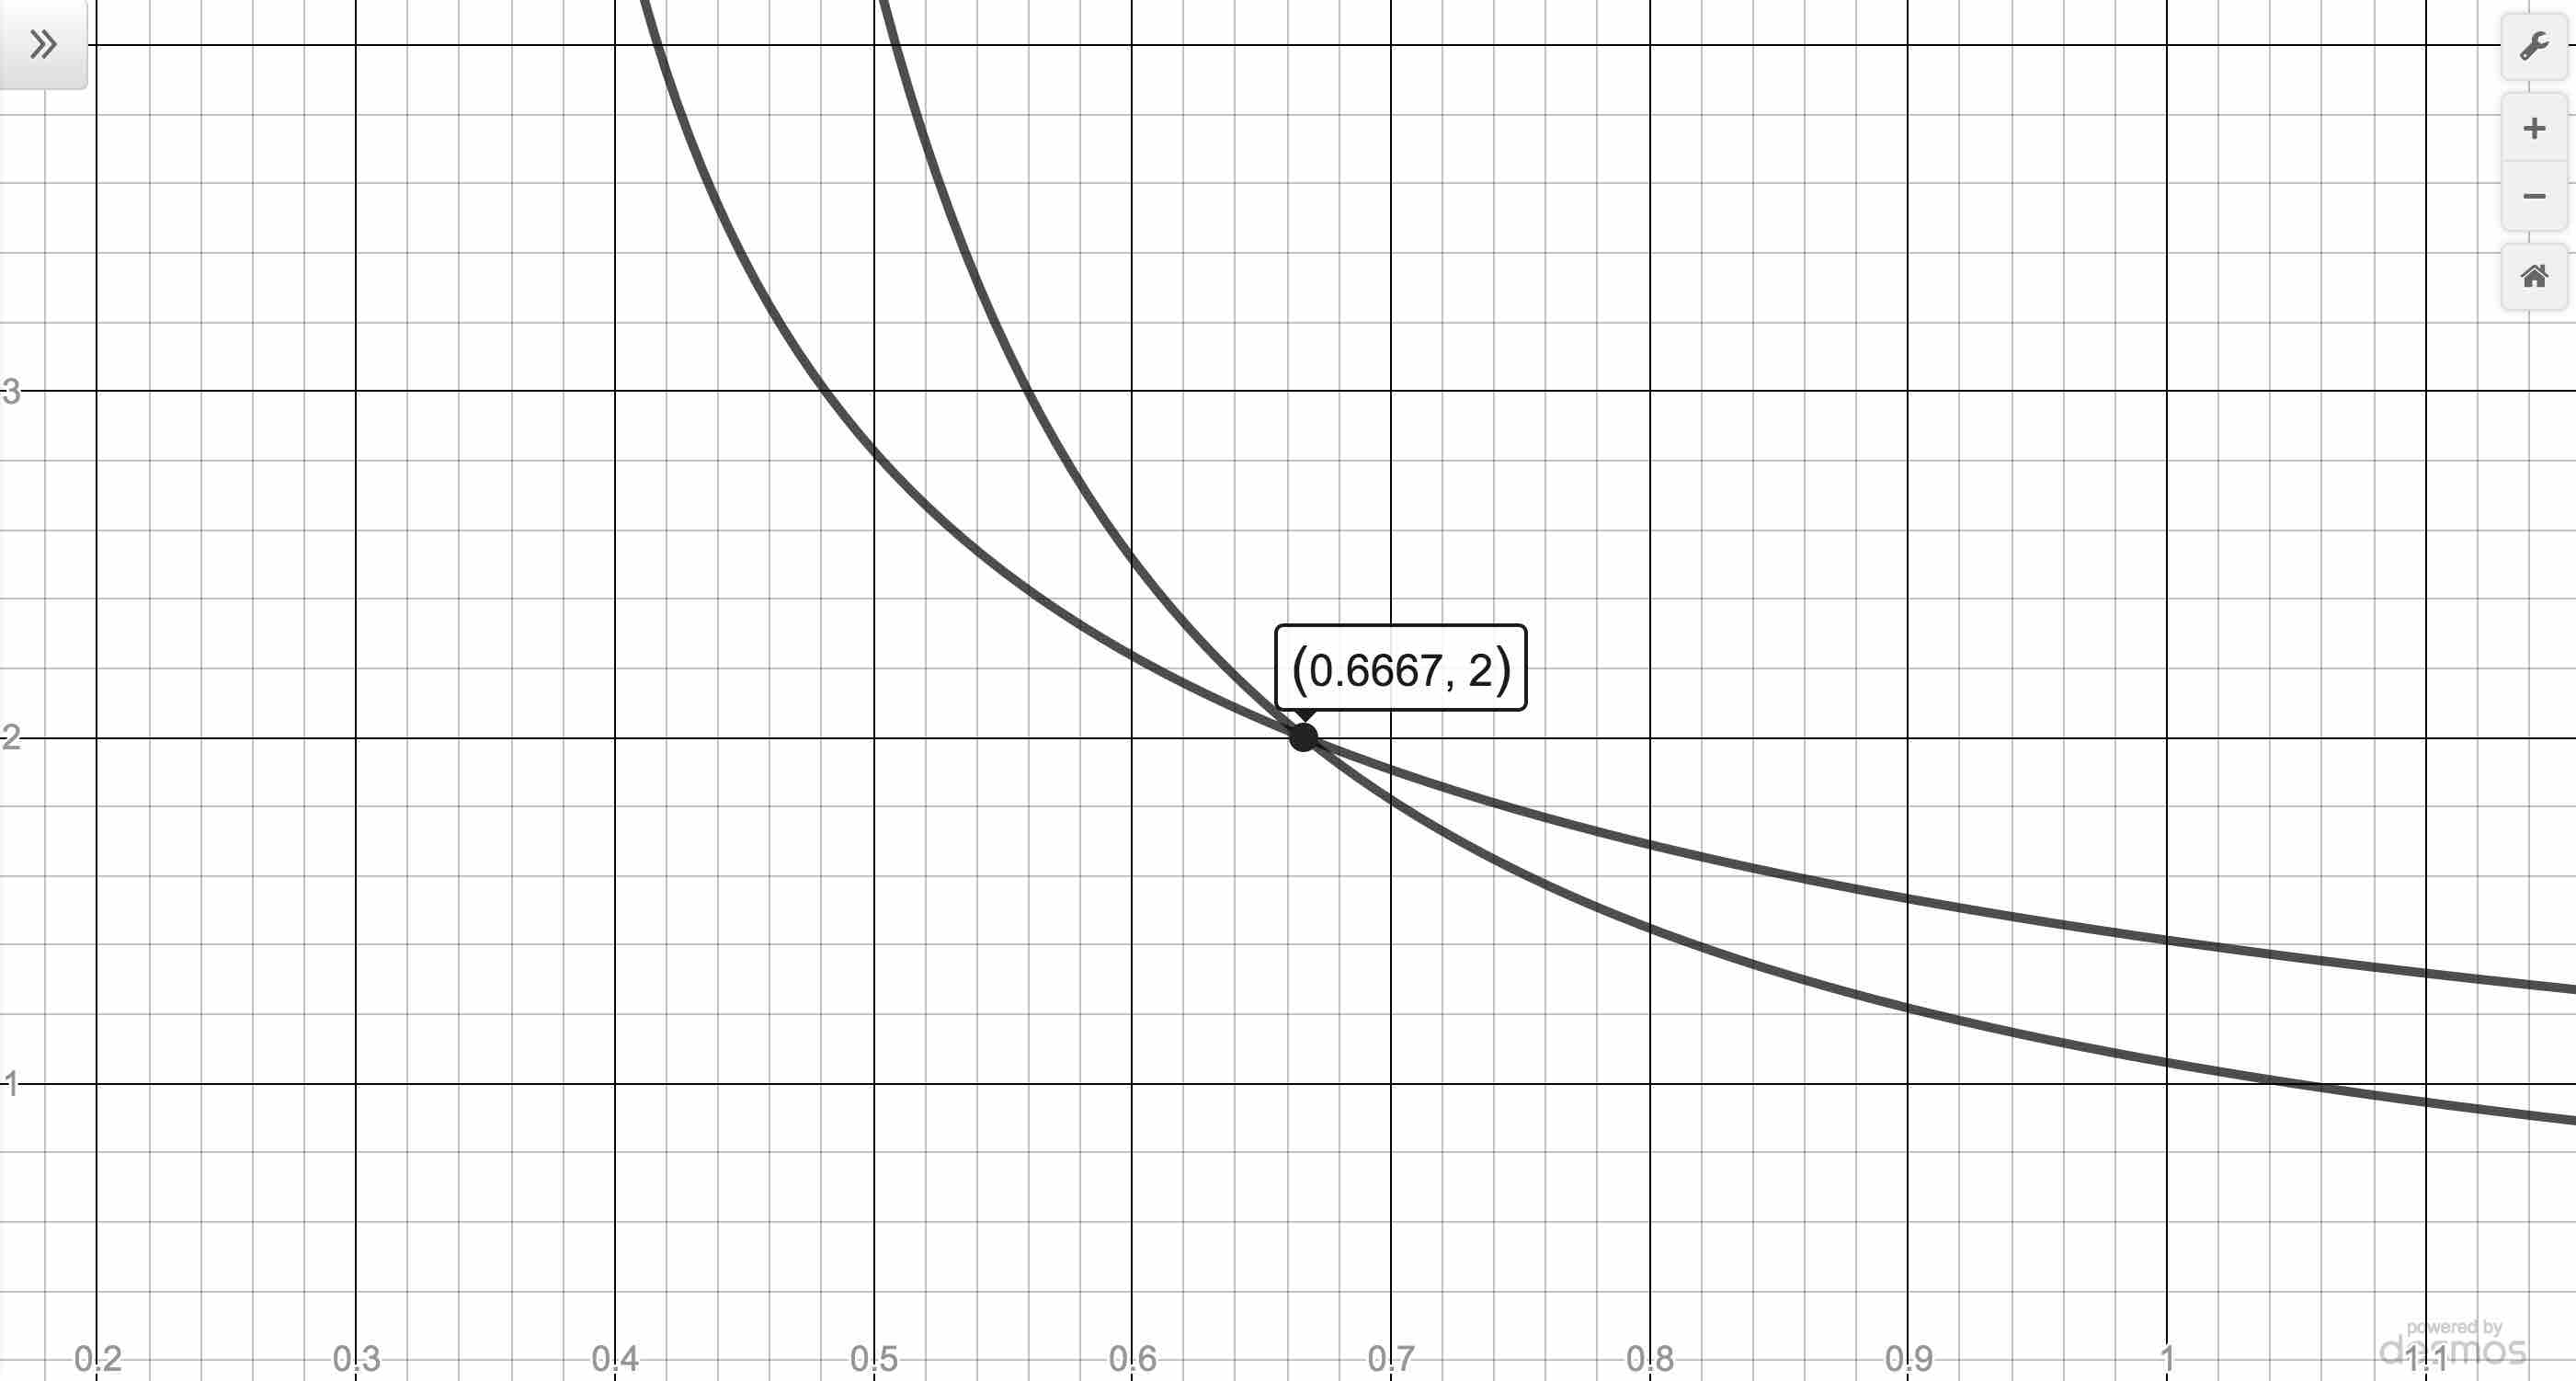
\includegraphics[width=3in]{./PowerEqIneqGraphics/PowerEqEx05.jpg} & 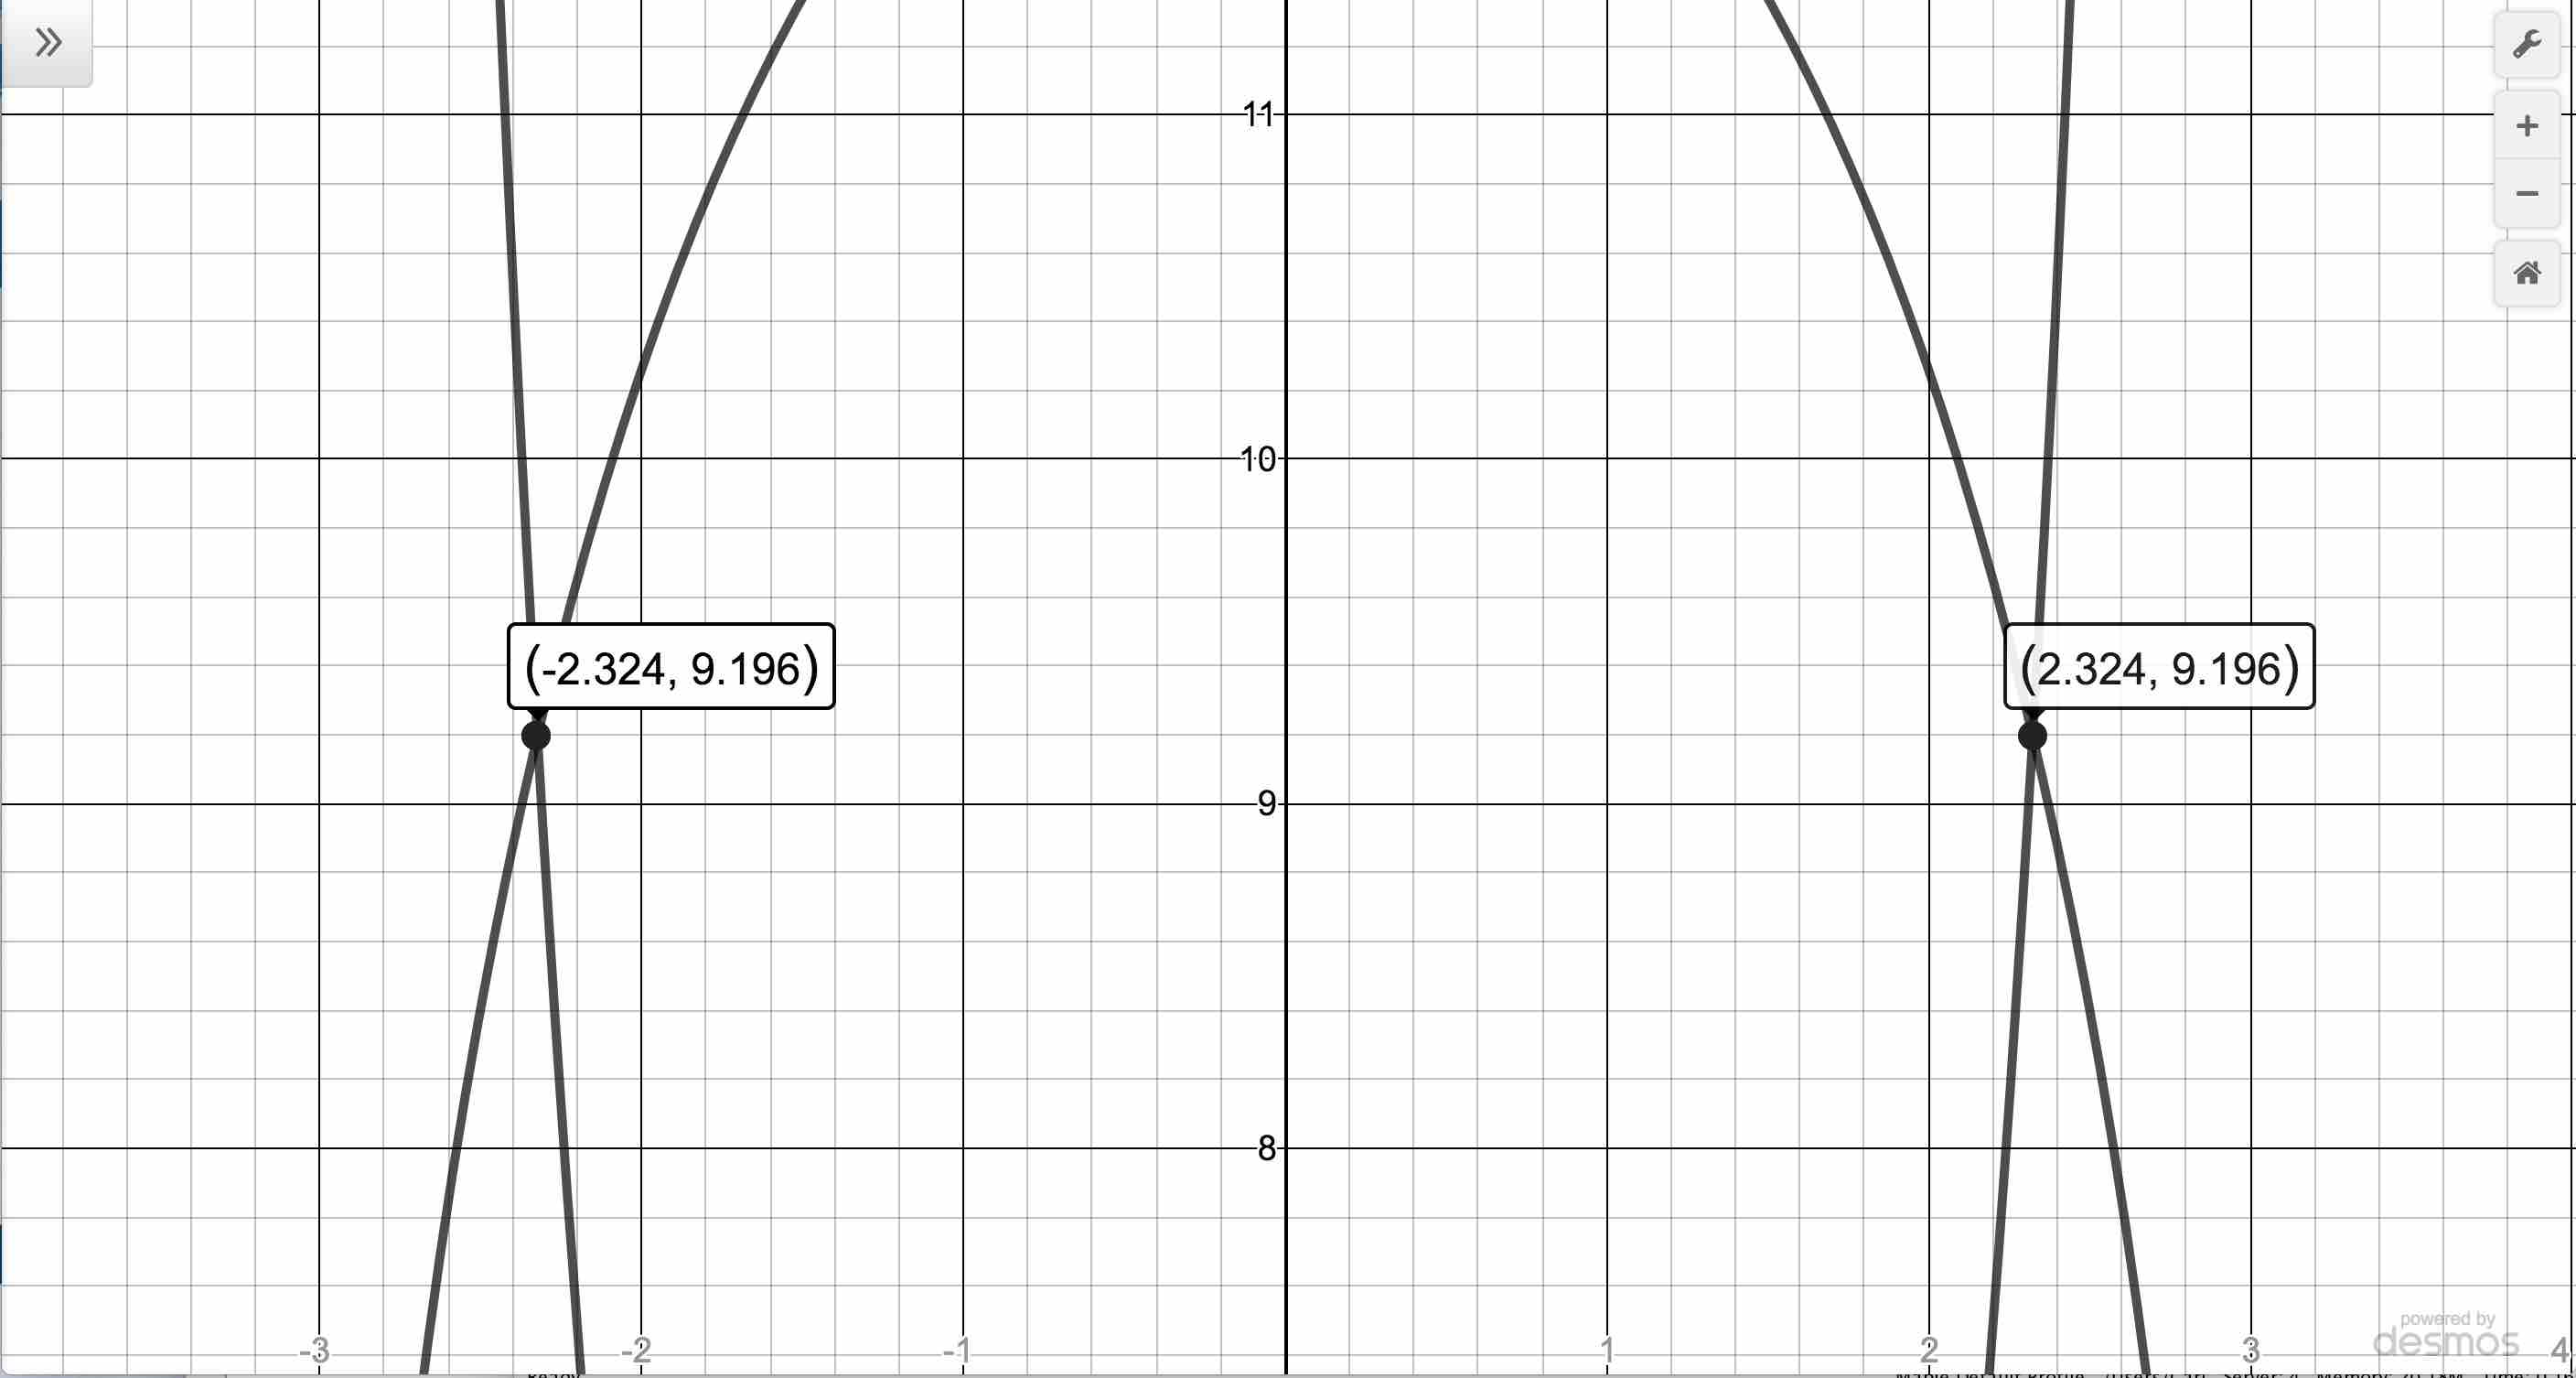
\includegraphics[width=3in]{./PowerEqIneqGraphics/PowerEqEx06.jpg} \\

Checking $2(3x-1)^{-0.5}  = 3x (3x-1)^{-1.5}$  & Checking  $6(9-t^2)^{\frac{1}{3}} = 4t^2 (9-x^2)^{\frac{2}{3}}$ \\

\end{tabular}

\end{center} 

\end{enumerate}

\qed

\end{example}

Note that Example \ref{powerequationex}, there are several ways to correctly solve each equation, and we endeavored to demonstrate a variety of methods.  For example, for number \ref{first}, instead of converting $(7-x)^{\frac{3}{2}}$ to a radical equation, we could use Theorem \ref{exponentprops}.  Since the root here ($2$) is even, we know $7-x \geq 0$ or $x \leq 7$.  Hence we may apply exponent properties: 

\[ \begin{array}{rclr}  

(7-x)^{\frac{3}{2}} & = & 8 & \\

 \left[(7-x)^{\frac{3}{2}}\right]^{\frac{2}{3}} & = & 8^{\frac{2}{3}} & \text{raise both sides to the $\frac{2}{3}$ power} \\
 
 (7-x)^{\frac{3}{2} \cdot \frac{2}{3}} & = & 4 & \text{Theorem \ref{exponentprops}} \\
 
(7-x)^{1} & = & 4 \\ \end{array} \]

from which we get $x = 3$.  If we try this same approach to solve number \ref{second}, however, we encounter difficulty.  From $(2t-1)^{\frac{2}{3}} -4 = 0$, we get $(2t-1)^{\frac{2}{3}}  =4$.  

\[ \begin{array}{rclr}  

(2t-1)^{\frac{2}{3}} & = & 4 & \\

 \left[(2t-1)^{\frac{2}{3}}  \right]^{\frac{3}{2}} & = & 4^{\frac{3}{2}}& \text{raise both sides to the $\frac{3}{2}$ power} \\ \end{array} \]
 
 Since the root here ($3$) is odd, we have no restriction on $2t-1$ but the exponent $\frac{3}{2}$ has an even denominator.  Hence, Theorem \ref{exponentprops} \textit{does not apply}.  That is, \[\left[(2t-1)^{\frac{2}{3}}  \right]^{\frac{3}{2}} \neq (2t-1)^{\frac{2}{3} \cdot \frac{3}{2}} = (2t-1)^{1} = (2t-1).\]
 Note that if we weren't careful, we'd have $2t-1 = 4^{\frac{3}{2}} = 8$ which gives $t= \frac{9}{2} = 4.5$ only.   We'd have missed the solution $t = -3.5$.  Truth be told, you \textit{can} simplify $\left[(2t-1)^{\frac{2}{3}}  \right]^{\frac{3}{2}} $ - just not using Theorem \ref{exponentprops}.  We leave it as an exercise to show  $\left[(2t-1)^{\frac{2}{3}}  \right]^{\frac{3}{2}} = |2t-1|$ and, more generally, $\left(x^{\frac{2}{3}}\right)^{\frac{3}{2}} = |x|$.
 
 Our next example is an application of the  \href{https://en.wikipedia.org/wiki/Cobb-Douglas_production_function}{\underline{Cobb Douglas}} production model of an economy.  The Cobb-Douglas model states that the yearly total dollar value of the production output in an economy is a function of \textit{two} variables:   labor (the total number of hours worked in a year) and capital (the total dollar value of the physical goods required for manufacturing.) The equation relating the production output level $P$, labor $L$ and capital $K$ takes the form $P = a L^{b} K^{1-b}$ where $0 < b < 1$; that is, the production level varies jointly with some power of the labor and capital.  

\begin{example} \label{CobbDouglasEx}  In their original paper \textit{A Theory of Production}\footnote{available \href{http://bit.ly/2dxlstt}{\underline{here}}.} Cobb and Douglas modeled the output of the US Economy (using 1899 as a baseline) using the formula $P = 1.01 L^{0.75} K^{0.25}$ where $P$, $L$, and $K$ were percentages of the 1899 figures for total production, labor, and capital, respectively.

\begin{enumerate}

\item  For 1910, the recorded labor and capital figures for the US Economy are $144 \%$ and $208 \%$ of the 1899 figures, respectively.  Find $P$ using these figures and interpret your answer.

\item  The recorded production value figure for 1920 is $231 \%$ of the 1899 figure.  Use this to write $K$ as a function of $L$, $K = f(L)$.  Find and interpret $f(193)$.

\item  Graph $K = f(L)$ and interpret the behavior as $L \rightarrow 0^{+}$ and $L \rightarrow \infty$.


\end{enumerate}

{\bf Solution.}

\begin{enumerate}

\item  In this case, $P = 1.01 L^{0.75} K^{0.25} = 1.01 (144)^{0.75} (208)^{0.25} \approx 159$ which means the dollar value of the total US Production in 1920 was approximately $159 \%$ of what it was in 1899.\footnote{This answer is remarkably accurate. Note:  all the dollar values here are recorded in `1880' dollars, per the source article. }  


\item We are given $P = 231 = 1.01L^{0.75} K^{0.25}$, so to write $K$ as a function of $L$, we need to solve this equation for $K$.  Since $L$ and $K$ are positive by definition, we can employ properties of exponents:

\[ \begin{array}{rclr}

231 & = & 1.01 L^{0.75} K^{0.25} & \\

\dfrac{231}{1.01 L^{0.75}} & = &  \dfrac{1.01 L^{0.75} K^{0.25}}{1.01 L^{0.75}} & \text{$L>0$, hence $L^{0.75} \neq 0$.}\\

K^{0.25} & = & 228.\overline{7128}L^{-0.75} & \text{rewrite} \\

\left(K^{0.25}\right)^{\frac{1}{0.25}} & = & \left(228.\overline{7128}L^{-0.75}\right)^{\frac{1}{0.25}} & \\

K^{\frac{0.25}{0.25}} & = & (228.\overline{7128})^{\frac{1}{0.25}} L^{-\frac{0.75}{0.25}} & \text{Theorem  \ref{exponentprops}} \\

K & = &  (228.\overline{7128})^{4} L^{-3} & \text{simplify} \\ \end{array} \]

Hence, $K = f(L) =  (228.\overline{7128})^{4} L^{-3}$ where $L>0$.  We find $f(193) =  (228.\overline{7128})^{4} (193)^{-3} \approx 381$ meaning that in order to maintain a production level of $231 \%$ of 1889 with a labor level at $193 \%$ of 1889, the required capital is $381 \%$ that of 1889.\footnote{The actual recorded figure is 407.}

\item The function $f(L)$ is a Laurent Monomial (see Section \ref{IntroRational}) with $n = 3$ and $a = (228.\overline{7128})^{4}$.  As such, as $L \rightarrow 0^{+}$, $f(L) \rightarrow \infty$.  This means that in order to maintain the given production level, as the available labor diminishes, the capital requirement become unbounded.  As $L \rightarrow \infty$, we have $f(L) \rightarrow 0$ meaning that as the available labor increases, the need for capital diminishes.  The graph of $f$ is called an `isoquant' - meaning `same quantity.'  In this context, the graph displays all combinations of labor and capital, $(L,K)$  which result in the \textit{same} production level, in this case, $231 \%$ of what was produced in 1889.

\begin{center}

\begin{mfpic}[25]{-1}{3}{-1}{3}
\axes
\scriptsize
\tlabel[cc](3, -0.5){$L$}
\tlabel[cc](-0.5, 3){$K$}
\tlabel[cc](2.5,1){$(1, (228.\overline{7128})^{4})$}
\normalsize
\penwd{1.25pt}
\arrow \reverse \arrow \function{0.7,2,0.1}{1/(x**3)}
\point[4pt]{(1,1)}
\tcaption{\scriptsize $K = f(L) =  (228.\overline{7128})^{4} L^{-3}$}
\end{mfpic}

\end{center}

\end{enumerate}

\qed

\end{example}

Next, we move on to solving inequalities with power functions.  As we've seen with other types of non-linear inequalities,\footnote{see Sections \ref{QuadraticFunctions}, \ref{RealZeros}, and \ref{RationalIneq}} an invaluable tool for us is the Sign Diagram.

\phantomsection
\label{algebraicsigndiagram}

%% \colorbox{ResultColor}{\bbm

\centerline{\textbf{Steps for Constructing a Sign Diagram for an Algebraic Function}} 

\medskip

\hspace{.17in} Suppose $f$ is an algebraic function. \index{sign diagram ! algebraic function}

\begin{enumerate}

\item  Place any values excluded from the domain of  $f$ on the number line with an `\textinterrobang' above them.

\item  Find the zeros of $f$ and place them on the number line with the number $0$ above them.

\item  Choose a test value in each of the intervals determined in steps 1 and 2.

\item  Determine and record the sign of $f(x)$ for each test value in step 3.

\end{enumerate}

%% \ebm}


As you may recall, since sign diagrams compare functions to $0$, the first step in solving inequalities using a sign diagram is to gather all the nonzero terms one one side of the inequality.  We demonstrate this technique in the following example.


\begin{example} \label{powerineqex} $~$

Solve the following inequalities.  Check your answers graphically with a calculator.

\begin{multicols}{2}
\begin{enumerate}

\item $2-\sqrt[4]{x+3} \geq 0$

\item $t^{2/3} < t^{4/3} - 6$


\setcounter{HW}{\value{enumi}}

\end{enumerate}
\end{multicols}

\begin{multicols}{2}
\begin{enumerate}

\setcounter{enumi}{\value{HW}}

\item  \label{third} $3 (2-x)^{\frac{1}{3}} \leq x (2-x)^{-\frac{2}{3}}$

\item \label{fourth} $(t-4)^{\frac{2}{3}} \geq -\dfrac{2t}{3(t-4)^{\frac{1}{3}}}$  


\end{enumerate}
\end{multicols}


{\bf Solution.}  

\begin{enumerate}

\item  To solve $2-\sqrt[4]{x+3} \geq 0$, it is tempting to rewrite this inequality as $2 \geq \sqrt[4]{x+3}$ and rid ourselves of the fourth root by raising both sides of this inequality to the fourth power.  While this technique works \textit{sometimes}, it doesn't work \textit{all} the time since raising both sides of an inequality to the fourth (more generally, to an even) power does not necessarily preserve inequalities .\footnote{For instance, $-2 \leq 1$ but $(-2)^{4} \geq (1)^2$.  We invite the reader to see what goes wrong if attempting to solve either of the following inequalities using this method: $-2 \geq \sqrt[4]{x+3}$, which has no solution, or  $-2 \leq \sqrt[4]{x+3}$, whose solution is $[-3,\infty)$.}  For that reason, we solve this inequality using a sign diagram since this technique will \textit{always} produce a correct solution.    

We already have all the nonzero terms on one side of the inequality, so we let $r(x) = 2-\sqrt[4]{x+3}$ and proceed to make a sign diagram.  Owing to the presence of the fourth root, we know $x+3 \geq 0$ or  $x \geq -3$.   Hence, we only concern ourselves with the portion of the number line representing $[3, \infty)$.  Next, we find the zeros of $r$ by solving $r(x) = 2-\sqrt[4]{x+3}=0$.  We get $\sqrt[4]{x+3} = 2$, so $x+3= 16$ and we get $x=13$.  We find this solution checks in our original equation,\footnote{Recall that raising both sides to an even power could produce extraneous solutions, so it is important we check here.}  and proceed to construct the sign diagram below on the left. Since we are looking for where $r(x) =  2-\sqrt[4]{x+3} \geq 0$, we are looking for the zeros of $r$ along with the intervals over which $r(x)$ is $(+)$.  We record our answer as $[-3, 13]$.  Below on the right is the graph of $y = 2-\sqrt[4]{x+3}$, and we can see that, indeed, the graph is above the $x$-axis ($y=0$) from $[-3, 13)$ and meets the $x$-axis at $x=13$, verifying our answer.

\begin{center}

\begin{tabular}{m{2in}m{2.5in}}

\begin{mfpic}[10]{0}{8}{-2}{2}

\arrow \polyline{(0,0), (8,0)}

\xmarks{0,4}

\tlabel[cc](0,-1){$-3 \hspace{7pt}$}

\tlabel[cc](2,1){$(+)$}

\tlabel[cc](4,-1){$13$}

\tlabel[cc](4,1){$0$}

\tlabel[cc](6,1){$(-)$}

\end{mfpic}

&

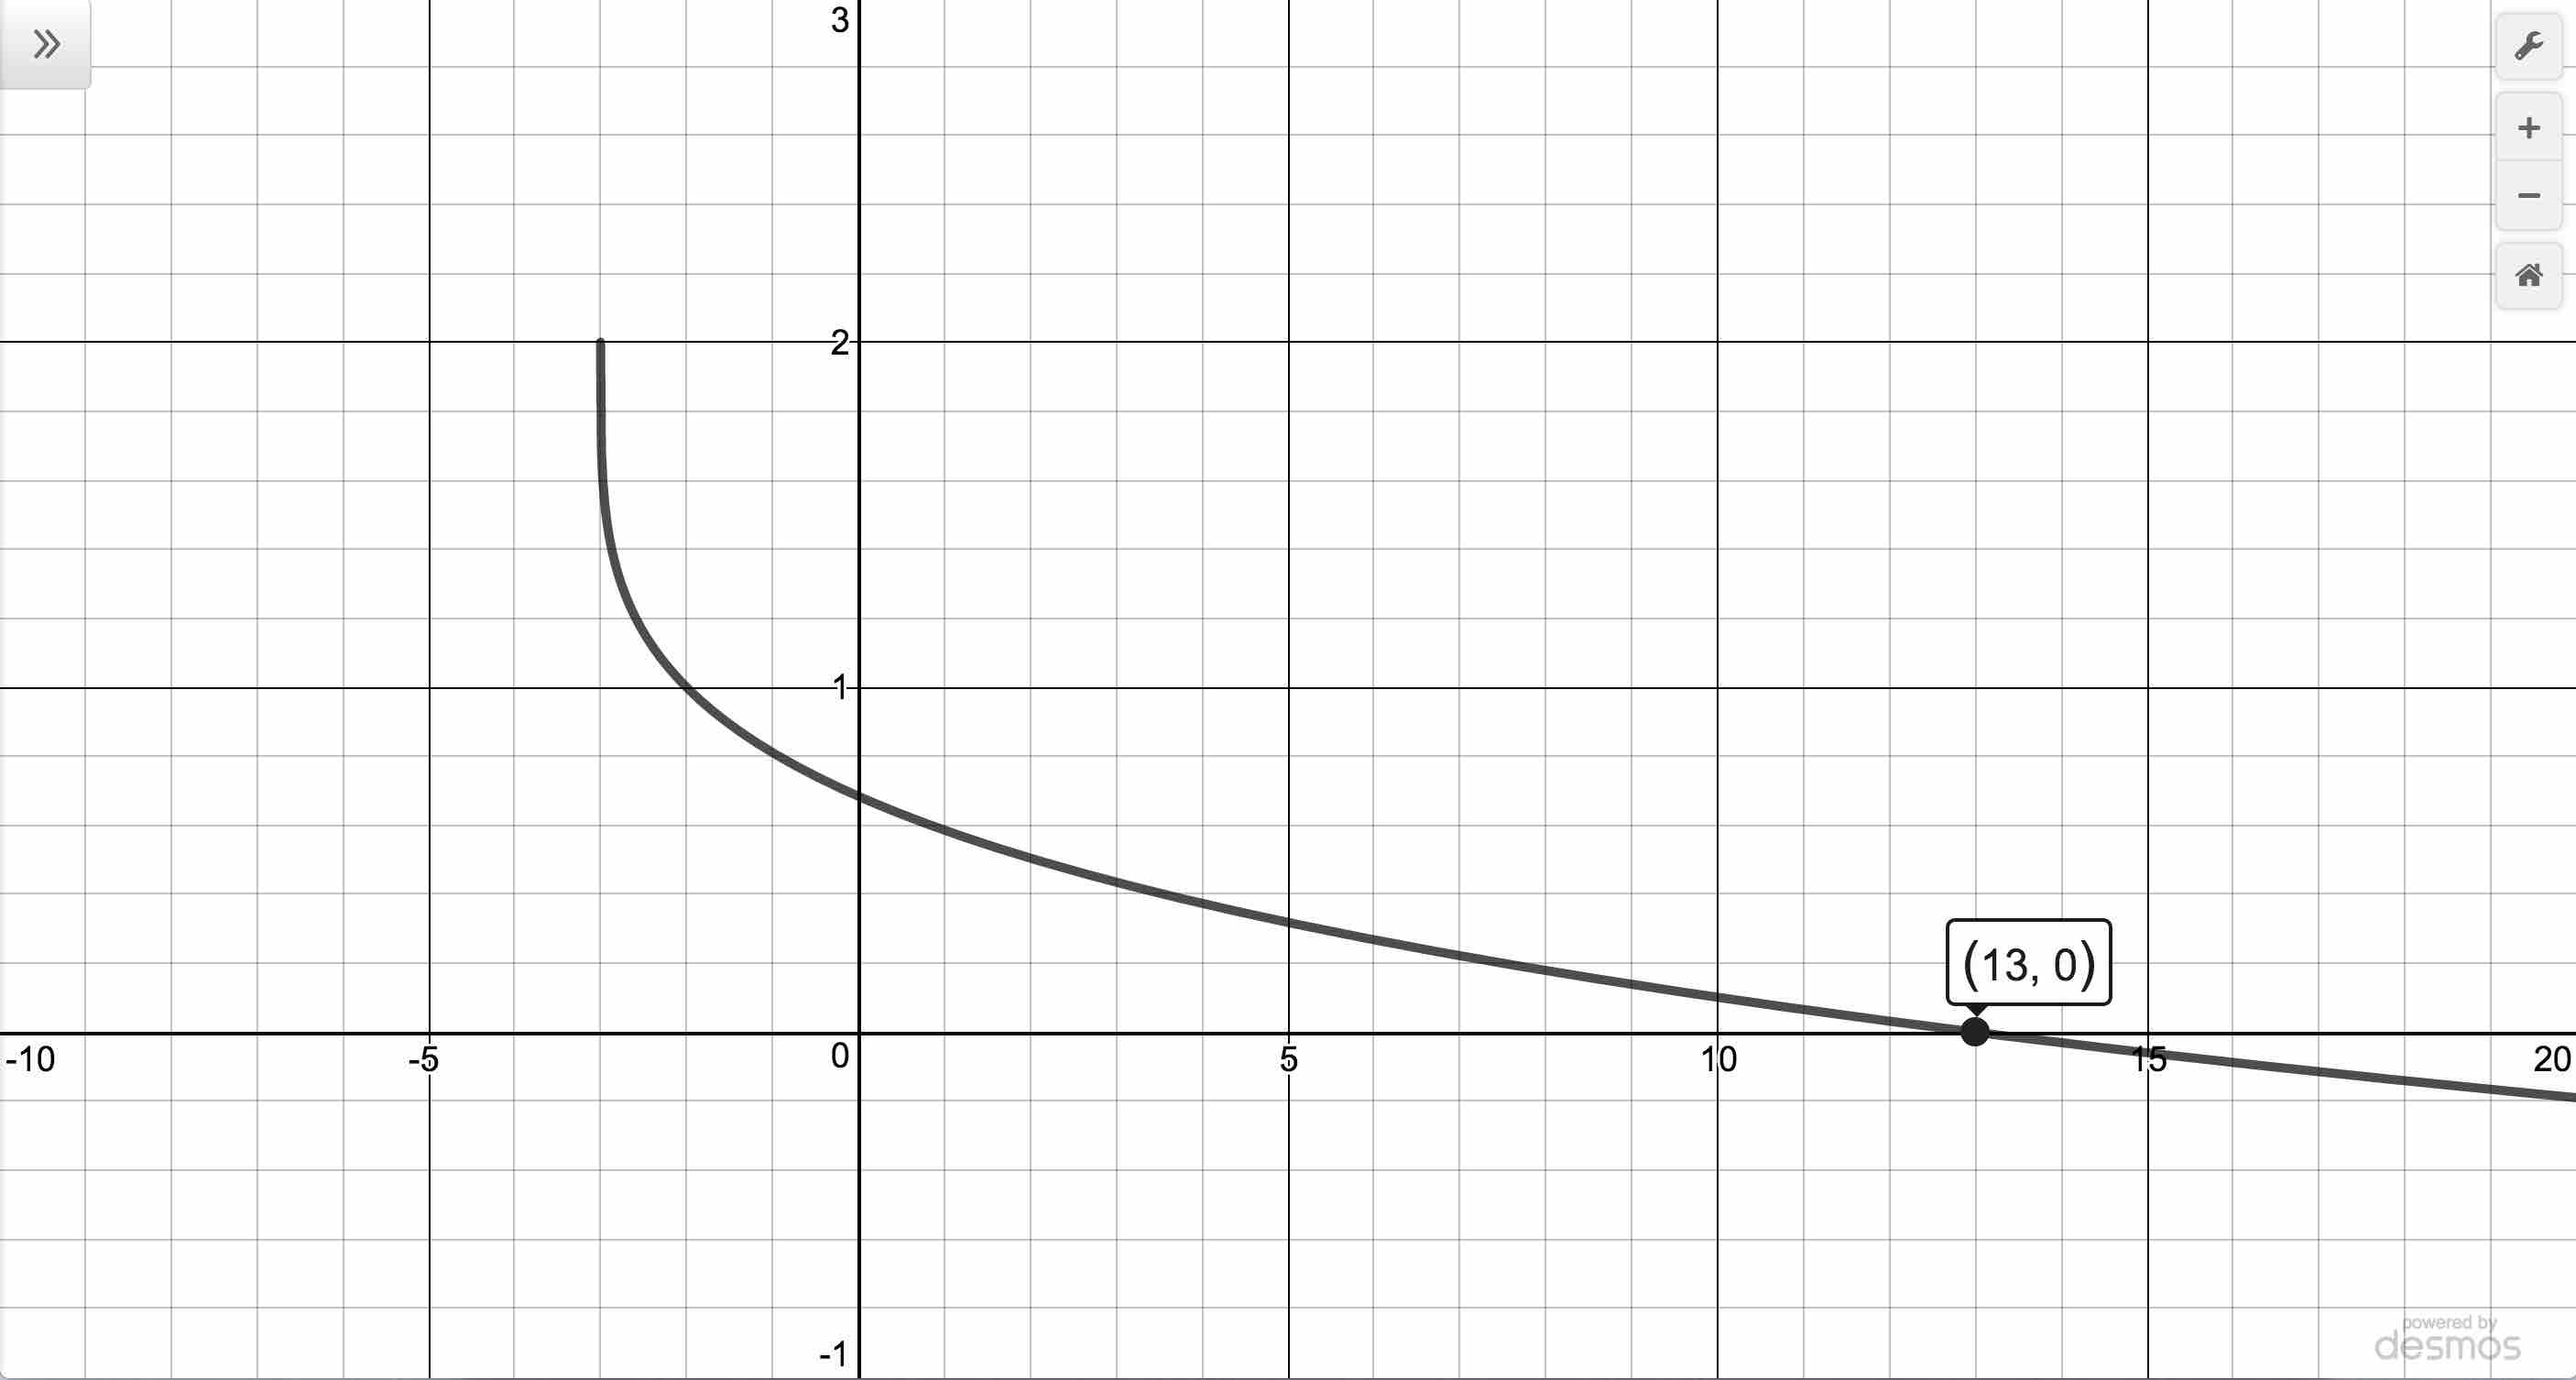
\includegraphics[width=3in]{./PowerEqIneqGraphics/PowerIneqEx01.jpg} \\ 

\end{tabular}

\end{center}

\item  To solve $t^{\frac{2}{3}} < t^{\frac{4}{3}} - 6$, we first rewrite as  $t^{\frac{4}{3}} -t^{\frac{2}{3}} - 6 > 0$.  We set $r(t) = t^{\frac{4}{3}} -t^{\frac{2}{3}} - 6$ and note that since the denominators in the exponents are $3$, they correspond to cube roots, which means the domain of $r$ is $(-\infty, \infty)$. To find the zeros for the sign diagram, we set $r(t) = 0$ and attempt to solve $t^{\frac{4}{3}} - t^{\frac{2}{3}} - 6 = 0$.   Since there are three terms, and the exponent on one of the variable terms, $t^{\frac{4}{3}}$, is exactly twice that of the other, $t^{\frac{2}{3}}$, we have ourselves a `quadratic in disguise.'   If we let $u = t^{\frac{2}{3}}$, then $u^2 = t^{\frac{4}{3}}$, so  in terms of $u$, we have $u^2 - u - 6 = 0$.  Solving  we get $u = -2$ or $u = 3$, hence  $t^{\frac{2}{3}} = -2$ or $t^{\frac{2}{3}} = 3$.  In root-power notation, these are $\sqrt[3]{t^2} = -2$ or $\sqrt[3]{t^2}= 3$.  Cubing both sides of these equations results in $t^2 = -8$, which admits no real solution, or $t^2 = 27$, which gives $t = \pm 3 \sqrt{3}$.  Using these zeros, we construct the sign diagram below on the left.  We find $r(t) = t^{\frac{4}{3}} -t^{\frac{2}{3}} - 6 > 0$  on $\left(-\infty, -3 \sqrt{3}\right)\cup \left(3 \sqrt{3}, \infty\right)$.  To check our answer graphically, we set $f(t) = t^{\frac{2}{3}}$ and $g(t) = t^{\frac{4}{3}}-6$.  The solution to  $t^{\frac{2}{3}} < t^{\frac{4}{3}} - 6$ corresponds to the inequality $f(t) < g(t)$, which means we are looking for the $t$ values for which the graph of $f$ is \textit{below} the graph of $g$.  On the graph below on the right, we see the graph of $f$ (the lighter colored curve) is below the graph of $g$ (the darker colored curve) for $t < - 5.196$ and again for $t > 5.196$, which are the grapher's approximations to $\pm 3 \sqrt{3}$.

\begin{center}

\begin{tabular}{m{2in}m{2.5in}}

\begin{mfpic}[10]{-5}{5}{-1}{2}

\arrow \reverse \arrow \polyline{(-5,0),(5,0)}

\xmarks{-2,2}

\tlabel[cc](-3.5,1){$(+)$}

\tlabel[cc](-2,-1){$-3 \sqrt{3} \hspace{7pt}$}

\tlabel[cc](-2,1){$0$}

\tlabel[cc](0,1){$(-)$}

\tlabel[cc](2,-1){$3 \sqrt{3}$}

\tlabel[cc](2,1){$0$}

\tlabel[cc](3.5,1){$(+)$}

\end{mfpic}

&

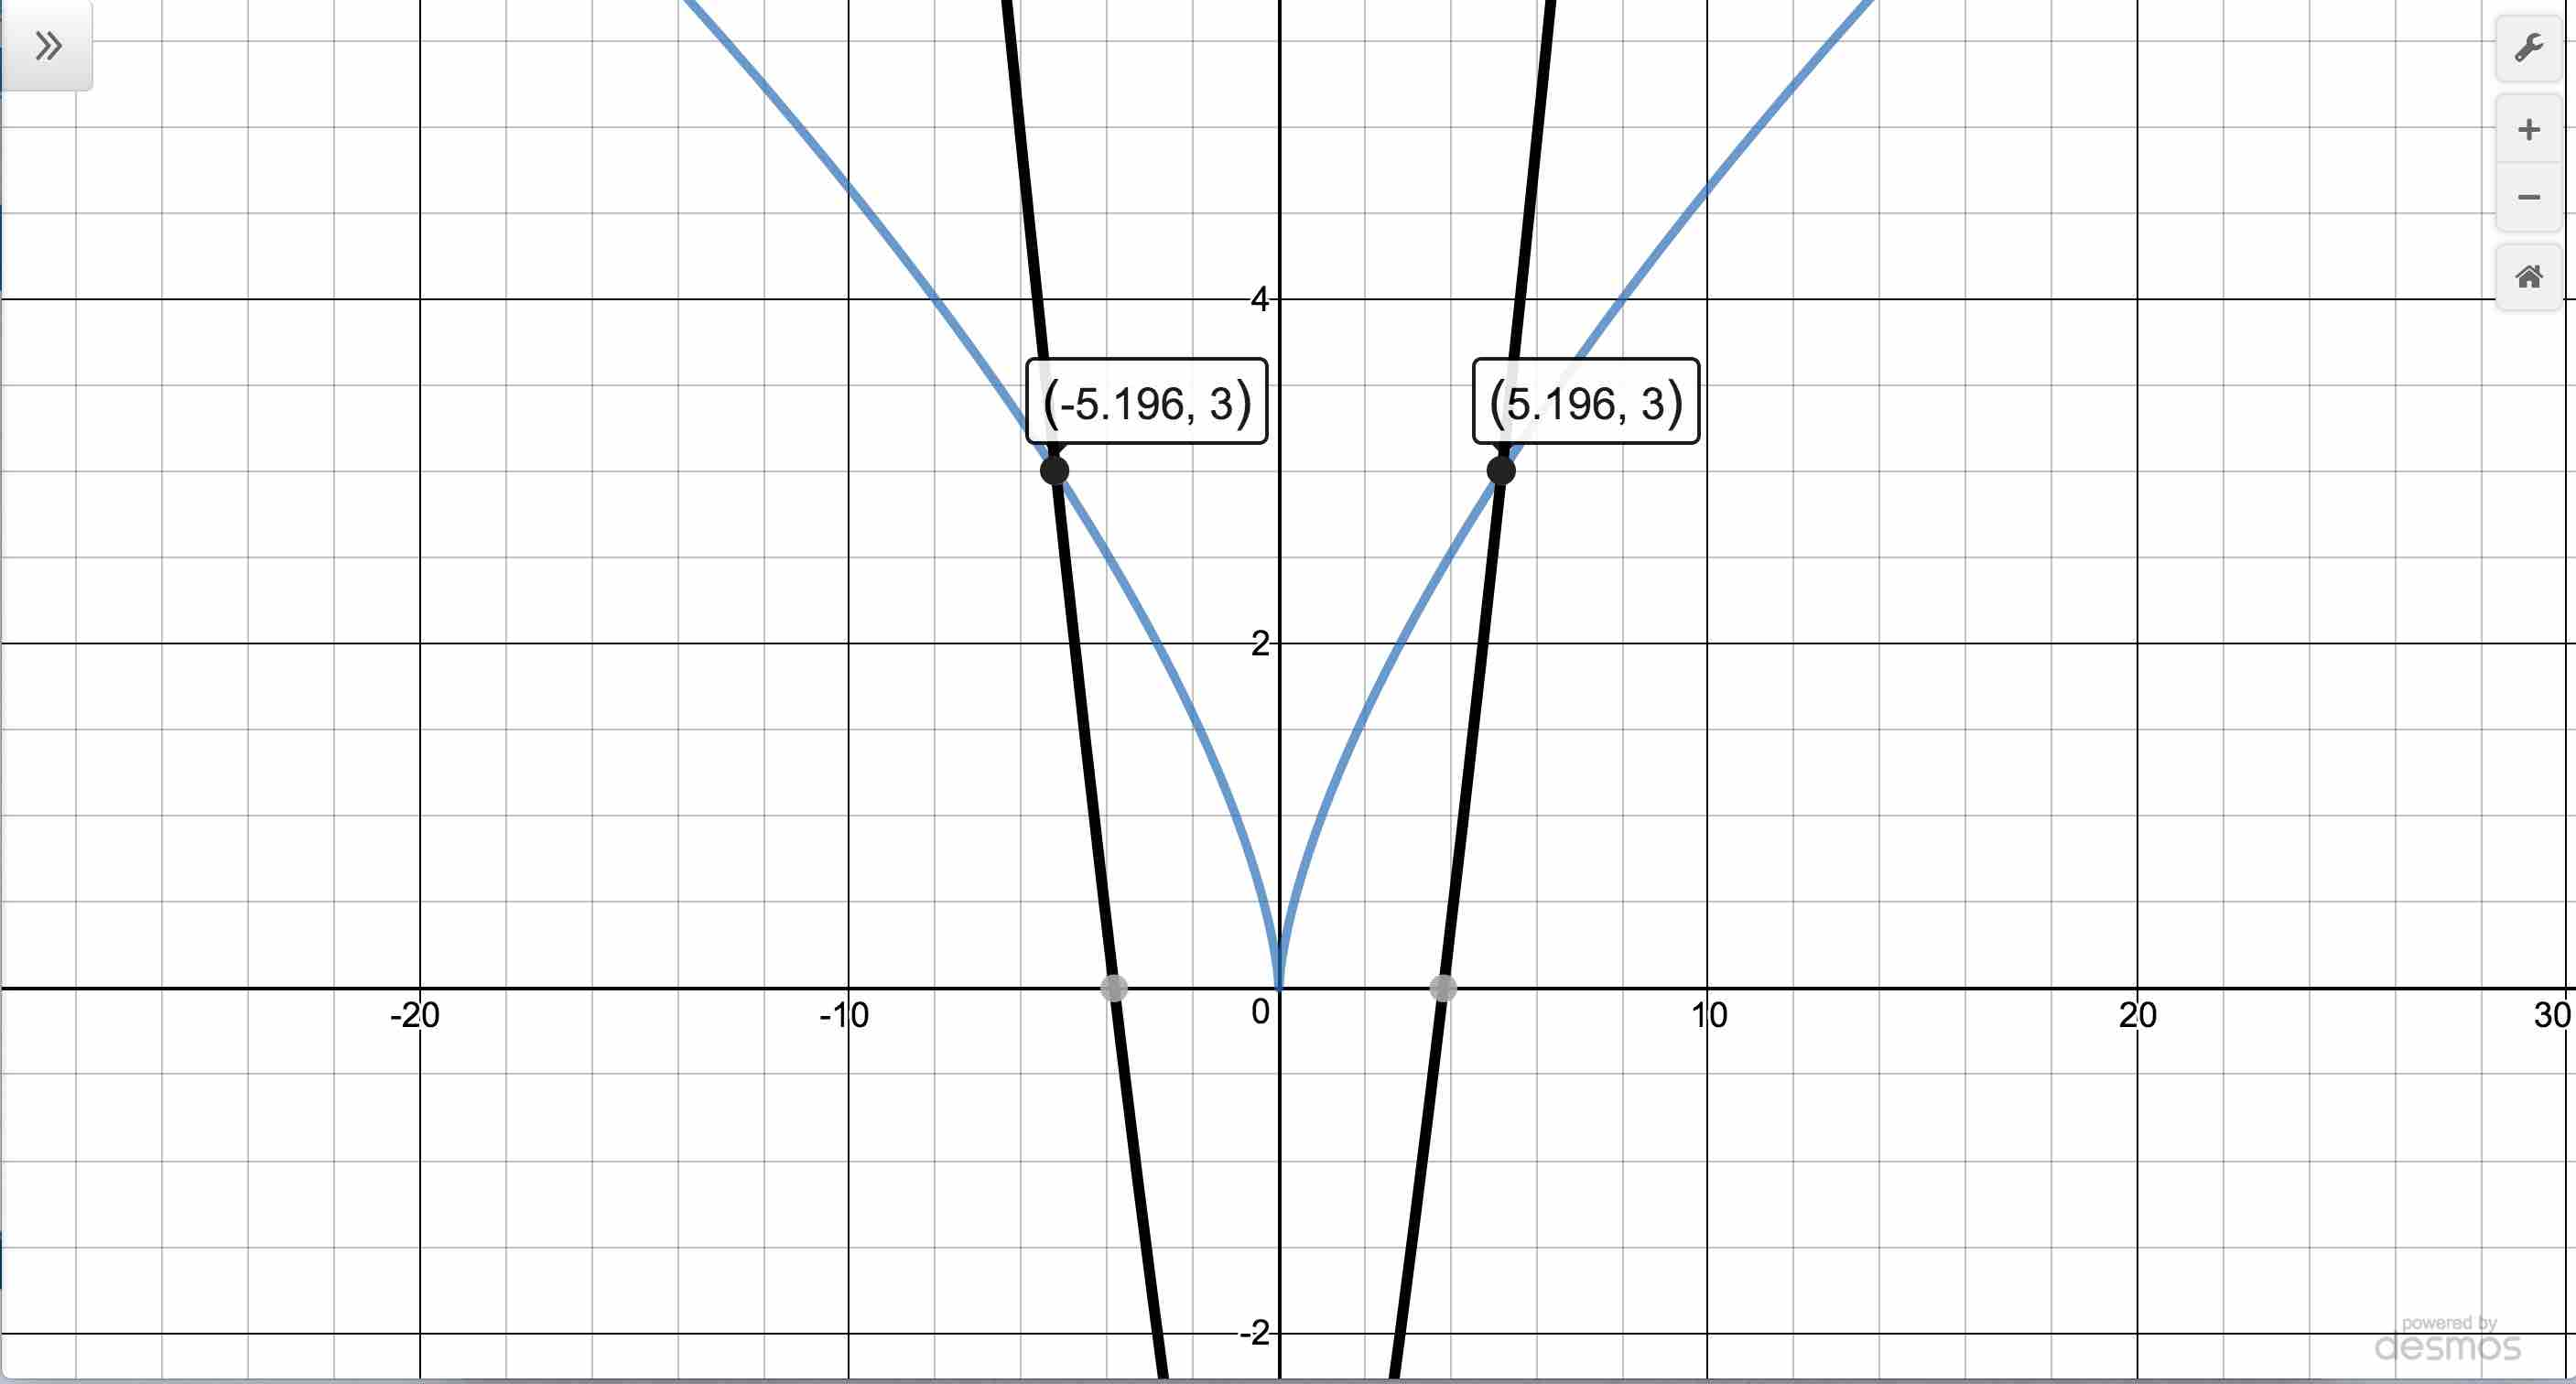
\includegraphics[width=3in]{./PowerEqIneqGraphics/PowerIneqEx02.jpg}  \\


\end{tabular}

\end{center}

\item  To solve $3 (2-x)^{\frac{1}{3}} \leq x (2-x)^{-\frac{2}{3}}$, we first gather all the nonzero terms to one side and obtain $3 (2-x)^{\frac{1}{3}} - x (2-x)^{-\frac{2}{3}} \leq 0$. Setting $r(x) = 3 (2-x)^{\frac{1}{3}} - x (2-x)^{-\frac{2}{3}}$, we note  since the denominators of the rational exponents are odd, we have no domain concerns owing to even indexed roots.  However, the negative exponent on the second term indicates a denominator.  Rewriting $r(x)$ with positive exponents, we obtain \[r(x) =  3 (2-x)^{\frac{1}{3}} - \frac{x}{(2-x)^{\frac{2}{3}}}\]  Setting the denominator equal to zero we get $(2-x)^{\frac{2}{3}} = 0$, which reduces to  $2-x=0$, or $x=2$.  Hence, the domain of $r$ is $(-\infty, 2) \cup (2, \infty)$. 

To find the zeros of $r$, we set $r(x) = 0$, so we set about solving \[3 (2-x)^{\frac{1}{3}} - \frac{x}{(2-x)^{\frac{2}{3}}} = 0.\] Clearing denominators, we get $3  (2-x)^{\frac{1}{3}} (2-x)^{\frac{2}{3}} - x = 0$.  Since the denominators of the exponents are odd, we may use Theorem \ref{exponentprops} to simplify this to $3(2-x)^{1} - x = 0$, and obtain $6-4x = 0$ or $x = \frac{3}{2}$.  In order for us to be able to more easily determine the sign of $r(x)$ at the test values, we rewrite $r(x)$ as a single term.\footnote{This also gives us a chance to review some good intermediate algebra!}  There are two schools of thought on how to proceed, so we demonstrate both.


\begin{itemize}

\item  \textit{Factoring Approach.}  From $r(x) = 3 (2-x)^{\frac{1}{3}} - x (2-x)^{-\frac{2}{3}}$, we note that the quantity $(2-x)$ is common to both terms.  When we factor out common factors, we factor out the quantity with the \textit{smaller} exponent.  In this case, since $-\frac{2}{3} < \frac{1}{3}$, we factor $(2-x)^{-\frac{2}{3}}$ from both quantities.  While it may seem odd to do so, we need to factor $(2-x)^{-\frac{2}{3}}$ \textit{from} $(2-x)^{\frac{1}{3}}$, which results in subtracting the exponent $-\frac{2}{3}$ from $\frac{1}{3}$.  We proceed using the usual properties of exponents.

\[ \begin{array}{rclr}

r(x)  & = & 3 (2-x)^{\frac{1}{3}} - x (2-x)^{-\frac{2}{3}} & \\ [3pt]
      & = & (2-x)^{-\frac{2}{3}} \left[ 3 (2-x)^{\frac{1}{3} - \left(-\frac{2}{3}\right)} - x\right] & \\ [6pt]
      & = & (2-x)^{-\frac{2}{3}}\left[3(2-x)^{\frac{3}{3}} - x\right] & \\ [3pt]
      & = & (2-x)^{-\frac{2}{3}}\left[3(2-x)^{1} - x\right] &  \\ [3pt]
      & = & (2-x)^{-\frac{2}{3}}\left(6-4x\right) & \\ [3pt]
      & = & (2-x)^{-\frac{2}{3}}\left(6-4x\right) & \\
      
\end{array}\]

Written without negative exponents, we have $r(x) = \dfrac{6-4x}{(2-x)^{\frac{2}{3}}}$.

\newpage

\item \textit{Common Denominator Approach.}  We rewrite 

\[ \begin{array}{rclr}

r(x)  & = & 3 (2-x)^{\frac{1}{3}} - x (2-x)^{-\frac{2}{3}} & \\ [3pt]
      & = & 3 (2-x)^{\frac{1}{3}} - \dfrac{x}{(2-x)^{\frac{2}{3}}} & \\ [10pt]
      & = & \dfrac{3 (2-x)^{\frac{1}{3}}(2-x)^{\frac{2}{3}}}{(2-x)^{\frac{2}{3}}} - \dfrac{x}{(2-x)^{\frac{2}{3}}} & \text{common denominator} \\ [10pt]
      & = & \dfrac{3 (2-x)^{\frac{1}{3} + \frac{2}{3}}}{(2-x)^{\frac{2}{3}}} - \dfrac{x}{(2-x)^{\frac{2}{3}}} & \text{Theorem \ref{exponentprops}}  \\ [10pt]
      & = & \dfrac{3 (2-x)^{\frac{3}{3}}}{(2-x)^{\frac{2}{3}}} - \dfrac{x}{(2-x)^{\frac{2}{3}}} & \\ [10pt]
      & = & \dfrac{3 (2-x)^1}{(2-x)^{\frac{2}{3}}} - \dfrac{x}{(2-x)^{\frac{2}{3}}} &  \\ [10pt]
      & = & \dfrac{3 (2-x) - x}{(2-x)^{\frac{2}{3}}} & \\ [10pt]
      & = & \dfrac{6-4x}{(2-x)^{\frac{2}{3}}} & \\

       
\end{array}\]


\end{itemize}

Using either approach, we end up with the same, simpler, expression for $r(x)$ and we use that to create our sign diagram as shown below on the left.  We find $r(x) \leq 0$ on $\left[\frac{3}{2},2\right) \cup (2, \infty)$.  To check this graphically, we set $f(x)=3 (2-x)^{\frac{1}{3}}$ (the lighter curve) and $g(x) = x (2-x)^{-\frac{2}{3}}$ (the darker curve). We confirm that the graphs intersect at $x=\frac{3}{2}$ and the graph of $f$ is below the graph of $g$ for $x > \frac{3}{2}$, with the exception of $x=2$ where it appears the graph of $g$ has a vertical asymptote. 

\begin{center}

\begin{tabular}{m{2in}m{2.5in}}

\begin{mfpic}[10]{-5}{5}{-1}{2}

\arrow \reverse \arrow \polyline{(-5,0),(5,0)}

\xmarks{-2,2}

\tlabel[cc](-3.5,1){$(+)$}

\tlabel[cc](-2,-1.25){$\frac{3}{2}$}

\tlabel[cc](-2,1){$0$}

\tlabel[cc](0,1){$(-)$}

\tlabel[cc](2,-1){$2$}

\tlabel[cc](2,1){\textinterrobang}

\tlabel[cc](3.5,1){$(-)$}

\end{mfpic}

&

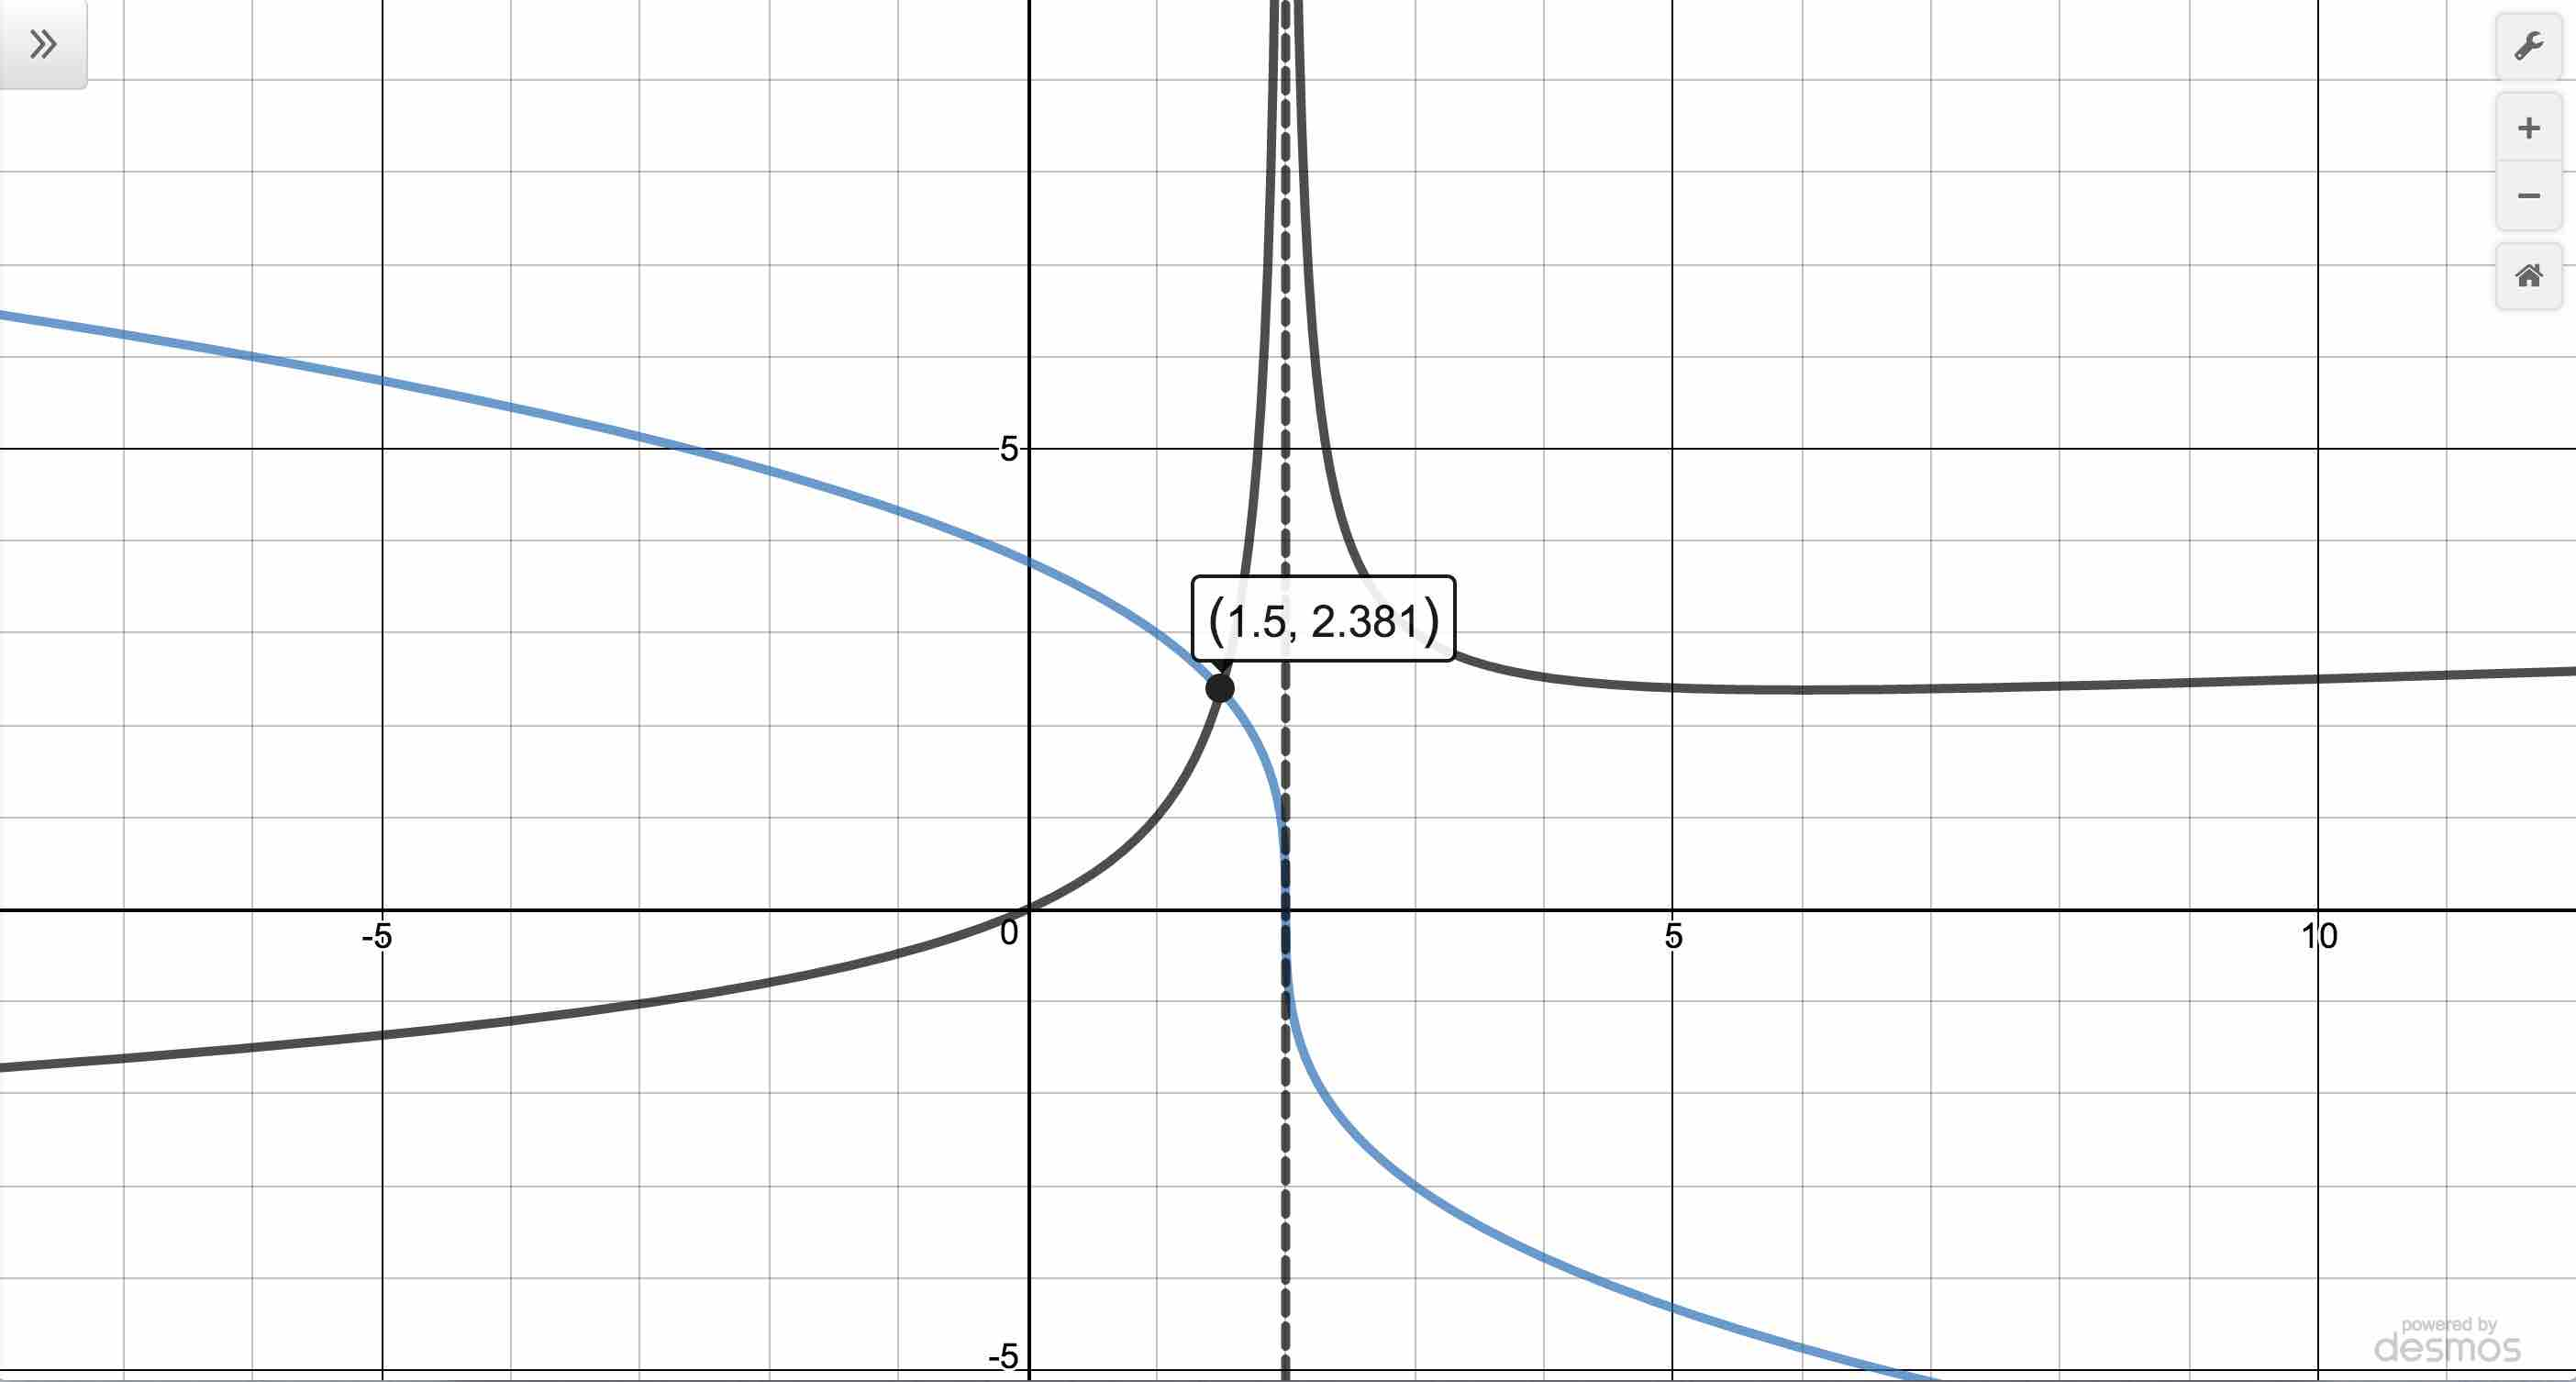
\includegraphics[width=3in]{./PowerEqIneqGraphics/PowerIneqEx03.jpg} \\


\end{tabular}

\end{center}


\item While it may be tempting to begin solving  our last inequality by clearing denominators, owing to the odd root, the quantity $3(t-4)^{\frac{1}{3}}$ can be both positive and negative for different values of $t$.  This means that if we chose to multiply both sides of our inequality by this quantity, we have no guarantee if the inequality would be preserved.  Hence we proceed as usual by gathering all the nonzero terms to one side, and,  with the ultimate goal of creating a sign diagram, get common denominators.  

\[ \begin{array}{rclr}

(t-4)^{\frac{2}{3}} & \geq &  - \dfrac{2t}{3(t-4)^{\frac{1}{3}}} & \\


(t-4)^{\frac{2}{3}} + \dfrac{2t}{3(t-4)^{\frac{1}{3}}}  & \geq & 0 \\

\dfrac{ (t-4)^{\frac{2}{3}} \cdot 3(t-4)^{\frac{1}{3}} }{3(t-4)^{\frac{1}{3}}}  + \dfrac{2t}{3(t-4)^{\frac{1}{3}}} & \geq & 0 & \text{common denominator} \\

\dfrac{3(t-4)^{\frac{2}{3}+\frac{1}{3}}}{3(t-4)^{\frac{1}{3}}}  + \dfrac{2t}{3(t-4)^{\frac{1}{3}}} & \geq & 0 & \text{Theorem \ref{exponentprops}} \\ 

\dfrac{3(t-4)^{1}}{3(t-4)^{\frac{1}{3}}}  + \dfrac{2t}{3(t-4)^{\frac{1}{3}}} & \geq & 0 & \\ 

\dfrac{3(t-4) + 2t}{3(t-4)^{\frac{1}{3}}}   & \geq & 0 & \\ 

\dfrac{5t-12}{3(t-4)^{\frac{1}{3}}}   & \geq & 0 & \\ 

\end{array} \]

We identify $r(t)$ as the left hand side of the inequality and see right away we must exclude $t=4$ from the domain owing to the quantity $(t-4)$ in the denominator.  As we have already mentioned, the root here ($3$) is odd, so we have no domain issues stemming from that.  To find the zeros of $r$, we set $r(t) = 0$ which quickly reduces to solving $5t-12 = 0$.  We get $t = \frac{12}{5}$.    From the sign diagram, we find $r(t) \geq 0$ on $\left(-\infty, \frac{5}{12} \right] \cup (4, \infty)$.  Graphing $f(t) = (t-4)^{\frac{2}{3}}$ (the lighter curve) and $g(t) = -\frac{2t}{3(t-4)^{\frac{1}{3}}}$ (the darker curve), we see the graph of $f$ is above the graph of $g$ for $t < 2.4$ and again for $t > 4$, with an intersection point at $t=2.4 = \frac{12}{5}$. 

\begin{center}

\begin{tabular}{m{2in}m{2.5in}}

\begin{mfpic}[10]{-5}{5}{-1}{2}

\arrow \reverse \arrow \polyline{(-5,0),(5,0)}

\xmarks{-2,2}

\tlabel[cc](-3.5,1){$(+)$}

\tlabel[cc](-2,-1.25){$\frac{12}{5}$}

\tlabel[cc](-2,1){$0$}

\tlabel[cc](0,1){$(-)$}

\tlabel[cc](2,-1){$4$}

\tlabel[cc](2,1){\textinterrobang}

\tlabel[cc](3.5,1){$(+)$}

\end{mfpic}

&

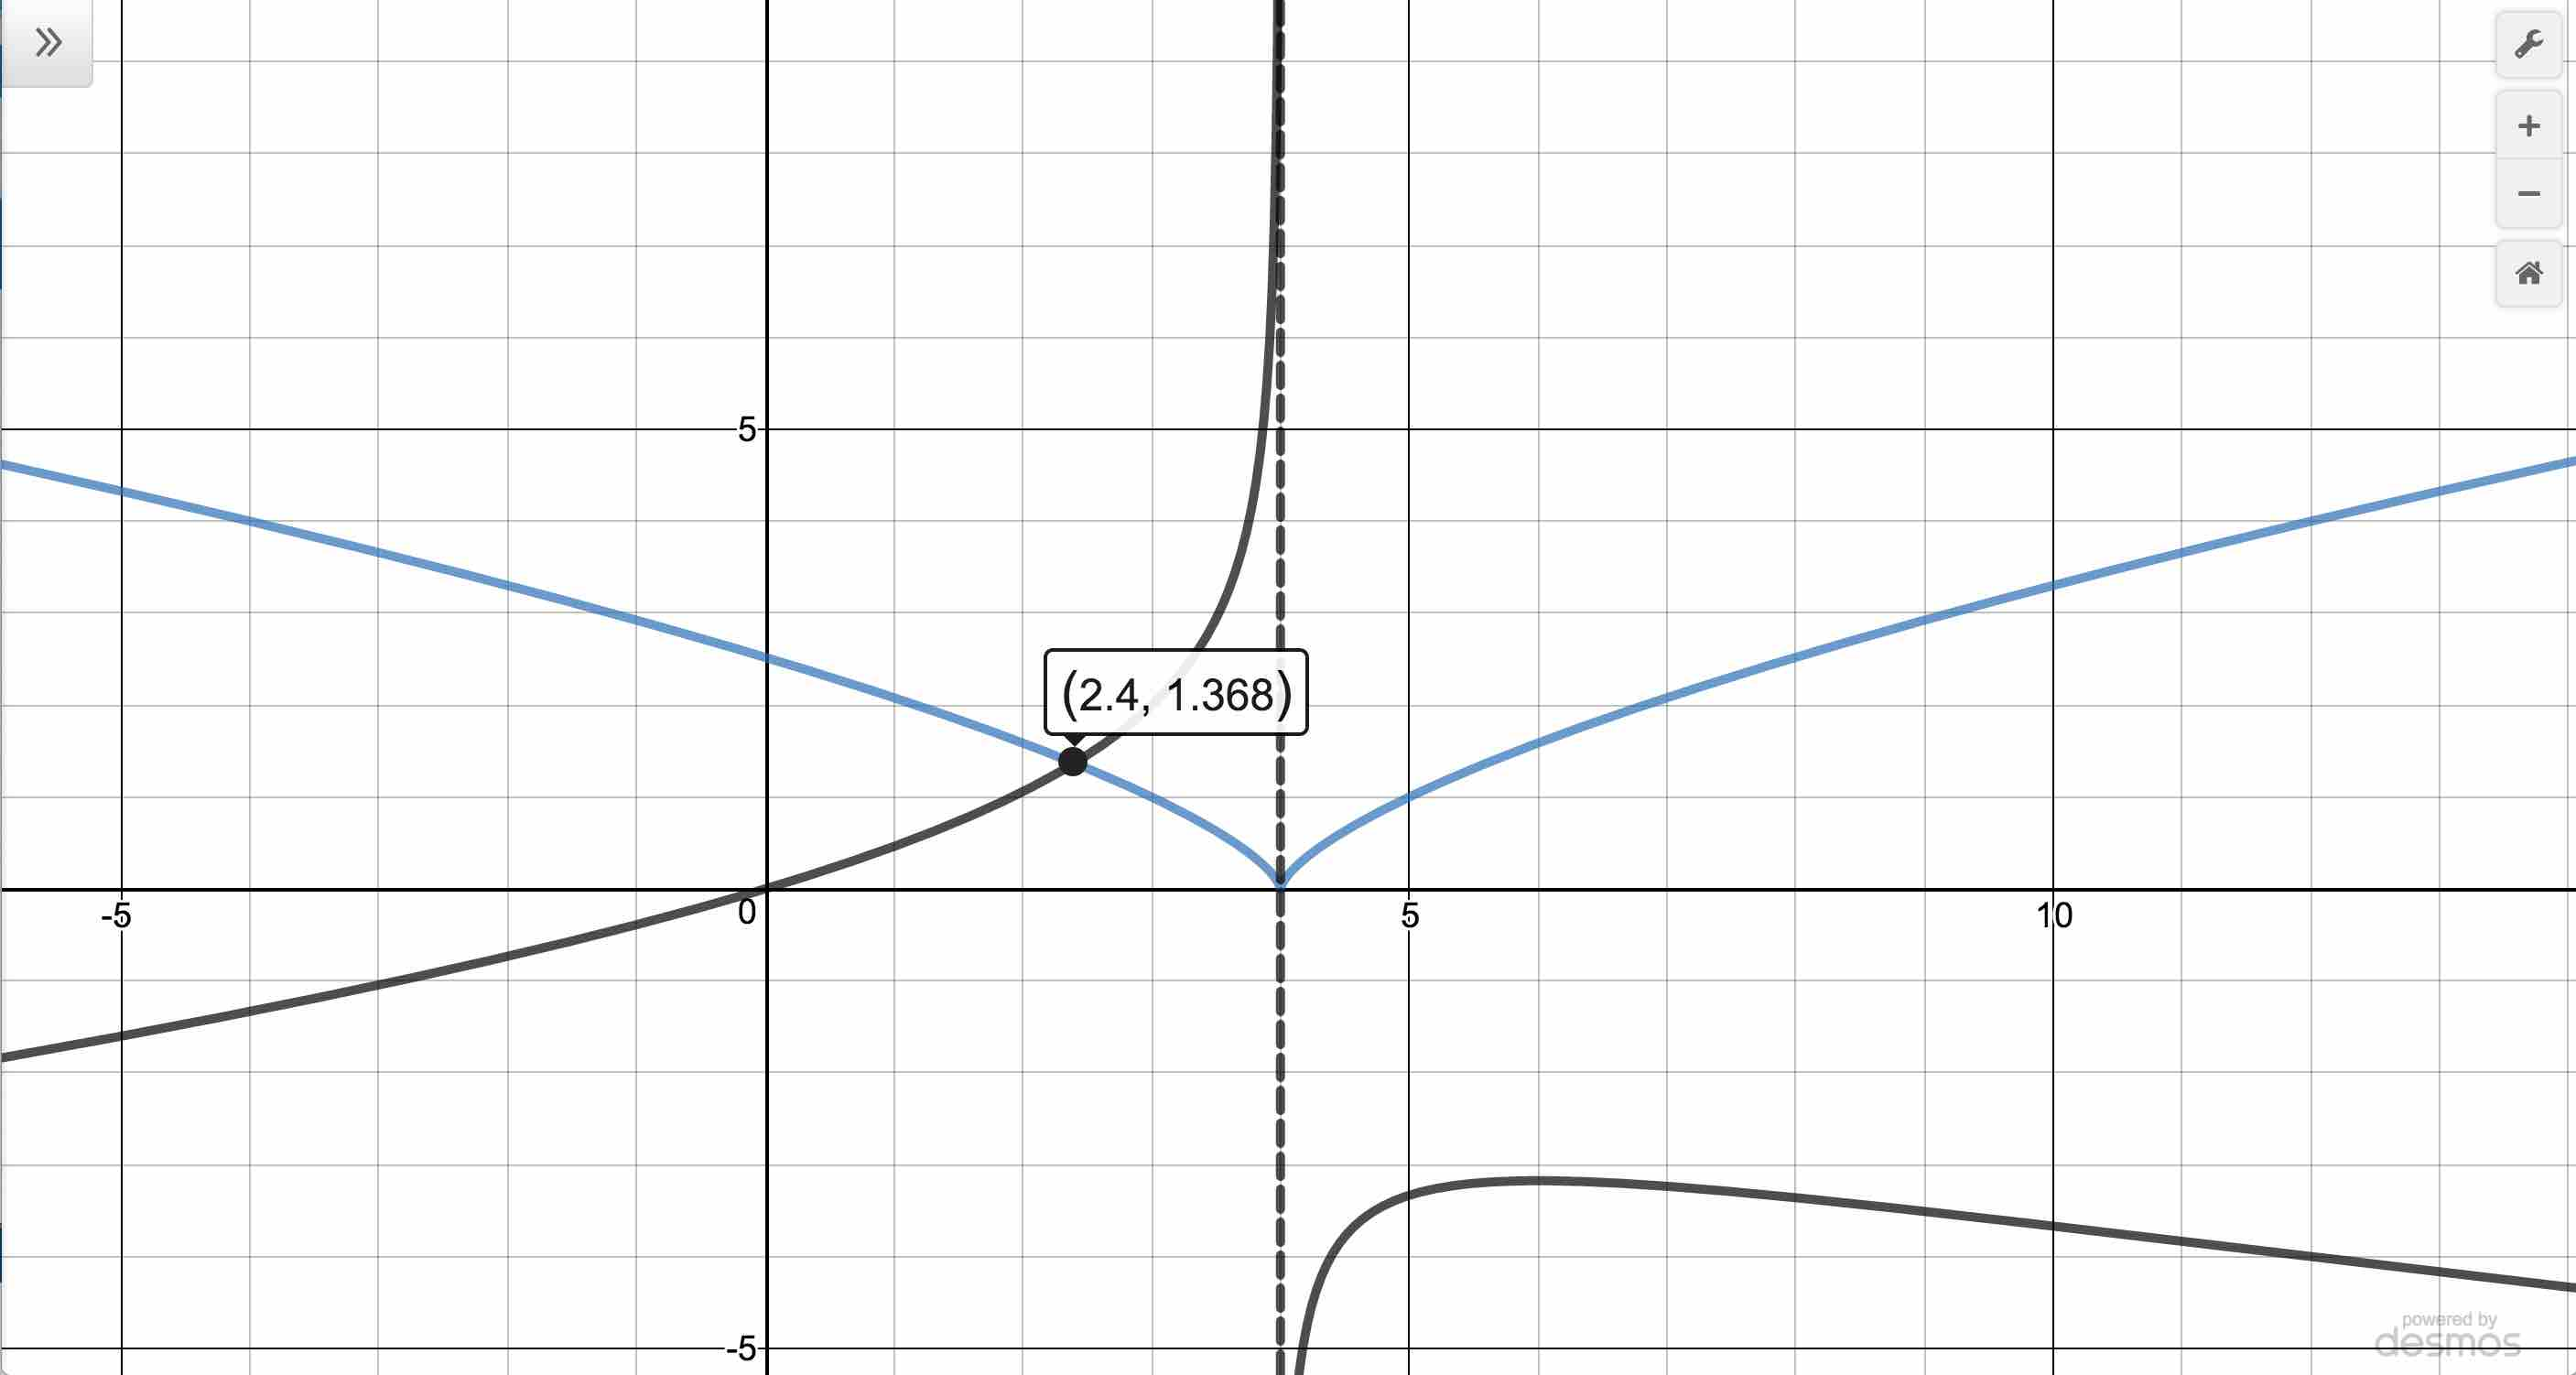
\includegraphics[width=3in]{./PowerEqIneqGraphics/PowerIneqEx04.jpg} \\


\end{tabular}

\end{center}



\end{enumerate}

\qed

\end{example}

\newpage

Note that in Example \ref{powerineqex} number \ref{third}, since $(2-x)^{\frac{2}{3}}$ is always positive  for $x \neq 2$ (owing to the squared exponent), we \textit{could} have short-cut the sign diagram, choosing to  clear denominators instead:

\[ \begin{array}{rclr}

3 (2-x)^{\frac{1}{3}} & \leq & x (2-x)^{-\frac{2}{3}} & \\

3 (2-x)^{\frac{1}{3}} & \leq & \dfrac{x}{(2-x)^{\frac{2}{3}}} & \\

\left[3 (2-x)^{\frac{1}{3}} \right] \left[  (2-x)^{\frac{2}{3}}\right]& \leq & \dfrac{x}{(2-x)^{\frac{2}{3}}}  \left[  (2-x)^{\frac{2}{3}}\right]&  \text{provided $x \neq 2$} \\
3 (2-x)^{\frac{1}{3}} (2-x)^{\frac{2}{3}} & \leq & x&  \\

3 (2-x)^{\frac{1}{3}+\frac{2}{3}} & \leq & x& \\

3(2-x) & \leq & x  & \\ \end{array} \]

Hence, we get $6-3x \leq x$ or $x \geq \frac{3}{2}$, provided $x \neq 2$. This matches our solution $\left[\frac{3}{2},2\right) \cup (2, \infty)$.  If, on the other hand, we tried this same manipulation with number \ref{fourth}, we would clear denominators, assuming $t \neq 4$ to obtain $3(t-4) \geq -2t$ or $t \geq \frac{12}{5}$ which is \textit{not} the correct solution.  The moral of the story is the more you understand, the less you need to rely on memorized processes and the more efficient your solution methodologies can become.  The sign diagram algorithm is a fail-safe method, but, in some cases, may be far from the most efficient one.  It's always best to understand the \textit{why} of a procedure as much as the \textit{how}.  

\newpage

\subsection{Exercises}

%% SKIPPED %% \documentclass{ximera}

\begin{document}
	\author{Stitz-Zeager}
	\xmtitle{TITLE}


In Exercises \ref{powereqineqexfirsta} - \ref{powereqineqexlasta}, solve the equation or inequality.  


\begin{multicols}{2}
\begin{enumerate}


\item $x+1 = (3x+7)^{\frac{1}{2}}$ \label{powereqineqexfirsta}
\item  $2x+1 = (3-3x)^{\frac{1}{2}}$

\setcounter{HW}{\value{enumi}}
\end{enumerate}
\end{multicols}

\begin{multicols}{2}
\begin{enumerate}
\setcounter{enumi}{\value{HW}}


\item  $t + (3t+10)^{0.5} = -2$
\item  $3t+(6-9t)^{0.5}=2$

\setcounter{HW}{\value{enumi}}
\end{enumerate}
\end{multicols}

\begin{multicols}{2}
\begin{enumerate}
\setcounter{enumi}{\value{HW}}

\item $x^{-1.5} = 8$
\item $2x - 1 =  (x + 1)^{-0.5}$

\setcounter{HW}{\value{enumi}}
\end{enumerate}
\end{multicols}

\begin{multicols}{2}
\begin{enumerate}
\setcounter{enumi}{\value{HW}}

\item $t^{\frac{2}{3}} = 4$
\item $(t - 2)^{\frac{1}{2}} + (t - 5)^{\frac{1}{2}} = 3$

\setcounter{HW}{\value{enumi}}
\end{enumerate}
\end{multicols}

\begin{multicols}{2}
\begin{enumerate}
\setcounter{enumi}{\value{HW}}

\item $(2x+1)^{\frac{1}{2}} = 3 + (4-x)^{\frac{1}{2}}$
\item  $5 - (4-2x)^{\frac{2}{3}} = 1$

\setcounter{HW}{\value{enumi}}
\end{enumerate}
\end{multicols}

\begin{multicols}{2}
\begin{enumerate}
\setcounter{enumi}{\value{HW}}

\item  $2t^{\frac{2}{3}} = 6 - t^{\frac{1}{3}}$  % $t=-8, \frac{27}{8}}$
\item  $2t^{\frac{1}{3}} = 1-3t^{\frac{2}{3}} $  % $t=-1, \frac{1}{27}$

\setcounter{HW}{\value{enumi}}
\end{enumerate}
\end{multicols}

\begin{multicols}{2}
\begin{enumerate}
\setcounter{enumi}{\value{HW}}

\item $2x^{1.5} = 15x^{0.75} + 8$  % $x=16$

\item  $35x^{-0.75} = x^{-1.5} +216$ % $x = \frac{1}{81}, \frac{1}{16}$

\setcounter{HW}{\value{enumi}}
\end{enumerate}
\end{multicols}

\begin{multicols}{2}
\begin{enumerate}
\setcounter{enumi}{\value{HW}}


\item  $10-\sqrt{t-2} \leq 11$ \vphantom{$t^{\frac{2}{3}} \leq 4$}
\item  $t^{\frac{2}{3}} \leq 4$ % $[-8,8]$

\setcounter{HW}{\value{enumi}}
\end{enumerate}
\end{multicols}

\begin{multicols}{2}
\begin{enumerate}
\setcounter{enumi}{\value{HW}}


\item  $\sqrt[3]{x} \leq x$   \vphantom{$(2-3x)^{\frac{1}{3}} > 3x$}
\item  $(2-3x)^{\frac{1}{3}} > 3x$  %$\left(-\infty, \frac{1}{3} \right)$

\setcounter{HW}{\value{enumi}}
\end{enumerate}
\end{multicols}

\begin{multicols}{2}
\begin{enumerate}
\setcounter{enumi}{\value{HW}}


\item  $(t^2-1)^{-\frac{1}{2}} \geq 2$  %$\left[ -\frac{\sqrt{5}}{2}, -1\right) \cup \left(1, \frac{\sqrt{5}}{2}\right]$
\item   $(t^2-1)^{-\frac{1}{3}} \leq 2$  %$\left[ -\frac{3\sqrt{2}}{4}, -1\right) \cup (-1,1) \cup \left(1, \frac{3\sqrt{2}}{4}\right]$

\setcounter{HW}{\value{enumi}}
\end{enumerate}
\end{multicols}

\begin{multicols}{2}
\begin{enumerate}
\setcounter{enumi}{\value{HW}}


\item  $3(x-1)^{\frac{1}{3}} +x (x-1)^{-\frac{2}{3}} \geq 0$ % $\left[ \frac{3}{4}, 1\right) \cup (1, \infty)$

\item $3(x-1)^{\frac{2}{3}} +2x (x-1)^{-\frac{1}{3}} \geq 0$ % $\left( -\infty, \frac{3}{5} \right] \cup (1, \infty)$

\setcounter{HW}{\value{enumi}}
\end{enumerate}
\end{multicols}


\begin{multicols}{2}
\begin{enumerate}
\setcounter{enumi}{\value{HW}}


\item  $2 (t-2)^{-\frac{1}{3}} -\frac{2}{3} t(t-2)^{-\frac{4}{3}} \leq 0$ \vphantom{$-\frac{4}{3} (t-2)^{-\frac{4}{3}} + \frac{8}{9} t (t-2)^{-\frac{7}{3}} \geq 0$}
\item  $-\frac{4}{3} (t-2)^{-\frac{4}{3}} + \frac{8}{9} t (t-2)^{-\frac{7}{3}} \geq 0$

\setcounter{HW}{\value{enumi}}
\end{enumerate}
\end{multicols}

\begin{multicols}{2}
\begin{enumerate}
\setcounter{enumi}{\value{HW}}


\item  $2x^{-\frac{1}{3}}(x-3)^{\frac{1}{3}} + x^{\frac{2}{3}} (x-3)^{-\frac{2}{3}} \geq 0$
\item $\sqrt[3]{x^{3} + 3x^{2} - 6x - 8} > x + 1$ \vphantom{ $2x^{-\frac{1}{3}}(x-3)^{\frac{1}{3}} + x^{\frac{2}{3}} (x-3)^{-\frac{2}{3}} \geq 0$}


\setcounter{HW}{\value{enumi}}
\end{enumerate}
\end{multicols}

\begin{multicols}{2}
\begin{enumerate}
\setcounter{enumi}{\value{HW}}

\item $4(7-t)^{0.75} - 3t(7-t)^{-0.25} \leq 0$  \vphantom{$4t^{0.75}(t - 3)^{-\frac{2}{3}} +9t^{-0.25}(t - 3)^{\frac{1}{3}} < 0$} %$[4, \infty)$

\item $4t^{0.75}(t - 3)^{-\frac{2}{3}} +9t^{-0.25}(t - 3)^{\frac{1}{3}} < 0$

\setcounter{HW}{\value{enumi}}
\end{enumerate}
\end{multicols}

\begin{enumerate}
\setcounter{enumi}{\value{HW}}


\item $x^{-\frac{1}{3}} (x-3)^{-\frac{2}{3}} - x^{-\frac{4}{3}} (x-3)^{-\frac{5}{3}} (x^2-3x+2) \geq 0$  \vphantom{$\frac{2}{3}(t + 4)^{\frac{3}{5}}(t - 2)^{-\frac{1}{3}} + \frac{3}{5}(t + 4)^{-\frac{2}{5}}(t - 2)^{\frac{2}{3}} \geq 0$ }
\item $\frac{2}{3}(t + 4)^{\frac{3}{5}}(t - 2)^{-\frac{1}{3}} + \frac{3}{5}(t + 4)^{-\frac{2}{5}}(t - 2)^{\frac{2}{3}} \geq 0$ \label{powereqineqexlasta}

\setcounter{HW}{\value{enumi}}
\end{enumerate}




\begin{enumerate}
\setcounter{enumi}{\value{HW}}
\item The Cobb-Douglas production model\footnote{See Example \ref{CobbDouglasEx} for more details on these sorts of models.} for the country of Sasquatchia is $P = 1.25L^{0.4}K^{0.6}$.  Here, $P$ represents the country's production (measured in thousands of Bigfoot  Bullion), $L$ represents the total labor (measured in thousands of hours) and $K$ represents the total investment in capital (measured in Bigfoot Bullion.)

\begin{enumerate}

\item \label{KintermsofLCobbexercise}Let $P = 300$ and solve for $K$ as a function of  $L$.  If $L = 100$, what is $K$?  Interpret each of the quantities in this case.

\item Graph your answer to \ref{KintermsofLCobbexercise} using a graphing utility.  What information does an ordered pair $(L, K)$ on this graph represent?  

\end{enumerate}

\end{enumerate}

\newpage

\subsection{Answers}

\begin{multicols}{3}
\begin{enumerate}


\item $x=3$  \vphantom{ $x = \frac{1}{4}$ }
\item  $x = \frac{1}{4}$
\item  $t=-3$  \vphantom{ $x = \frac{1}{4}$ }

\setcounter{HW}{\value{enumi}}
\end{enumerate}
\end{multicols}

\begin{multicols}{3}
\begin{enumerate}
\setcounter{enumi}{\value{HW}}


\item  $t = -\frac{1}{3}, \; \frac{2}{3}$  \vphantom{$x = \frac{\sqrt{3}}{2}$}
\item $x = \frac{1}{4}$  \vphantom{$x = \frac{\sqrt{3}}{2}$}
\item $x = \frac{\sqrt{3}}{2}$

\setcounter{HW}{\value{enumi}}
\end{enumerate}
\end{multicols}

\begin{multicols}{3}
\begin{enumerate}
\setcounter{enumi}{\value{HW}}


\item $t = \pm 8$
\item $t = 6$
\item  $x = 4$

\setcounter{HW}{\value{enumi}}
\end{enumerate}
\end{multicols}

\begin{multicols}{3}
\begin{enumerate}
\setcounter{enumi}{\value{HW}}
 
\item  $x=-2, 6$  \vphantom{$t=-8, \frac{27}{8}$}
\item   $t=-8, \frac{27}{8}$
\item   $t=-1, \frac{1}{27}$   \vphantom{$t=-8, \frac{27}{8}$}

\setcounter{HW}{\value{enumi}}
\end{enumerate}
\end{multicols}

\begin{multicols}{3}
\begin{enumerate}
\setcounter{enumi}{\value{HW}}

\item $x=16$ \vphantom{$x = \frac{1}{81}, \frac{1}{16}$}
\item  $x = \frac{1}{81}, \frac{1}{16}$
\item  $[2, \infty)$   \vphantom{$x = \frac{1}{81}, \frac{1}{16}$}


\setcounter{HW}{\value{enumi}}
\end{enumerate}
\end{multicols}

\begin{multicols}{3}
\begin{enumerate}
\setcounter{enumi}{\value{HW}}

\item  $[-8,8]$    \vphantom{ $\left(-\infty, \frac{1}{3} \right)$}
\item  $[-1, 0] \cup [1, \infty)$  \vphantom{ $\left(-\infty, \frac{1}{3} \right)$}
\item $\left(-\infty, \frac{1}{3} \right)$

\setcounter{HW}{\value{enumi}}
\end{enumerate}
\end{multicols}

\begin{multicols}{2}
\begin{enumerate}
\setcounter{enumi}{\value{HW}}

\item $\left[ -\frac{\sqrt{5}}{2}, -1\right) \cup \left(1, \frac{\sqrt{5}}{2}\right]$
\item  $\left(-\infty, -\frac{3\sqrt{2}}{4} \right] \cup (-1,1) \cup \left[ \frac{3\sqrt{2}}{4}, \infty \right)$

\setcounter{HW}{\value{enumi}}
\end{enumerate}
\end{multicols}

\begin{multicols}{2}
\begin{enumerate}
\setcounter{enumi}{\value{HW}}


\item   $\left[ \frac{3}{4}, 1\right) \cup (1, \infty)$

\item $\left( -\infty, \frac{3}{5} \right] \cup (1, \infty)$

\setcounter{HW}{\value{enumi}}
\end{enumerate}
\end{multicols}

\begin{multicols}{2}
\begin{enumerate}
\setcounter{enumi}{\value{HW}}

\item  $(-\infty, 2) \cup (2,3]$
\item  $(2,6]$

\setcounter{HW}{\value{enumi}}
\end{enumerate}
\end{multicols}

\begin{multicols}{2}
\begin{enumerate}
\setcounter{enumi}{\value{HW}}

\item $(-\infty, 0) \cup [2,3) \cup (3, \infty)$
\item $(-\infty, -1)$  


\setcounter{HW}{\value{enumi}}
\end{enumerate}
\end{multicols}

\begin{multicols}{2}
\begin{enumerate}
\setcounter{enumi}{\value{HW}}

\item $[4,7)$  \vphantom{$\left(0, \frac{27}{13} \right)$}
\item $\left(0, \frac{27}{13} \right)$

\setcounter{HW}{\value{enumi}}
\end{enumerate}
\end{multicols}

\begin{multicols}{2}
\begin{enumerate}
\setcounter{enumi}{\value{HW}}
\item $(-\infty, 0) \cup (0,3)$   \vphantom{$(-\infty, -4) \cup \left(-4, -\frac{22}{19}\right] \cup (2, \infty)$}
\item $(-\infty, -4) \cup \left(-4, -\frac{22}{19}\right] \cup (2, \infty)$

\setcounter{HW}{\value{enumi}}
\end{enumerate}
\end{multicols}

\begin{enumerate}
\setcounter{enumi}{\value{HW}}
\item \begin{enumerate}

\item $K=f(L) = (240)^{ \frac{5}{3}} L^{- \frac{2}{3}}$.  $f(100)  \approx 430.2148$.  This means in order for the production level of Sasquatchia to reach 300,000 Bigfoot Bullion with a labor investment of 100,000 hours, the country needs to invest approximately 430 Bigfoot Bullion into capital.


\item If a point $(L,K)$ is on the graph of this function, it means a combination of $L$ thousand hours of labor with an investment of $K$ Bigfoot Bullion into the Sasquatian Economy will result in a production level of 300,000 Bigfoot Bullion.

\centerline{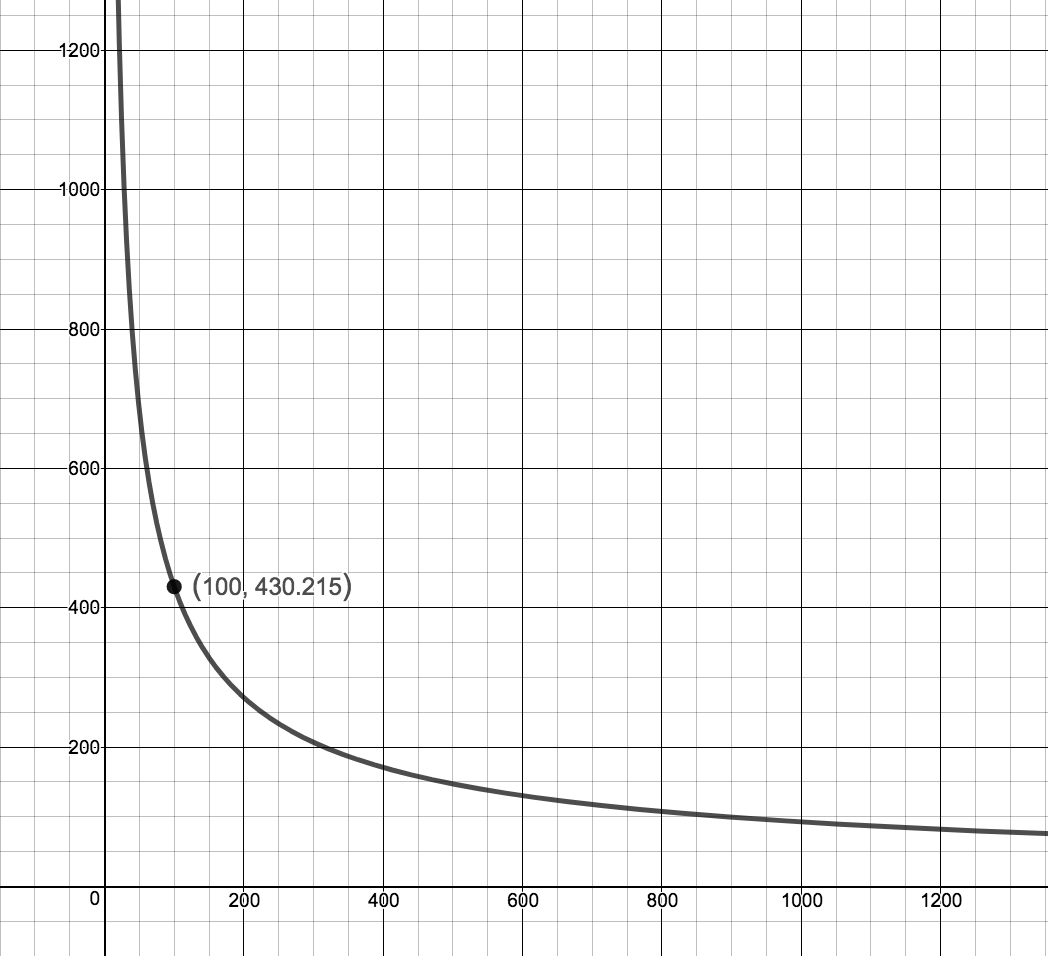
\includegraphics[height=2in]{./PowerEqIneqGraphics/CobbDouglasExercise.jpg}}



\end{enumerate}

\end{enumerate}

\end{document}


\closegraphsfile

\end{document}
